\documentclass[UTF8]{ctexart}
\usepackage[table]{xcolor}
\usepackage{bm}
\usepackage{amssymb}
\usepackage{mathtools}
\usepackage{amsmath}
\usepackage{float}
\usepackage{rotating}
\usepackage{booktabs}
\usepackage{pdfpages}
\usepackage{subfigure}
\usepackage{mathtools}
\usepackage{amsmath}
\usepackage{listings}
\usepackage{fancybox}
%\usepackage{xcolor}
%\usepackage{colortbl}
\usepackage{diagbox}
\usepackage{amssymb}
\usepackage{warpcol}
\usepackage{lscape}
\usepackage[framemethod=tikz]{mdframed}
\usepackage{longtable,booktabs}
\definecolor{ocre}{RGB}{243,102,25}
\definecolor{mygray}{RGB}{243,243,244}


\lstset{
columns=flexible,
numbers=left,
numberstyle=\footnotesize\color{darkgray}, 
basicstyle=\small\ttfamily,
stringstyle=\color{purple},
keywordstyle=\color[RGB]{40,40,255}\bfseries,
commentstyle=\it\color[RGB]{0,96,96},  
stringstyle=\rmfamily\slshape\color[RGB]{128,0,0}, 
showstringspaces=false,      
% directivestyle=\color{blue},
frame=shadowbox,
%framerule=0pt,
backgroundcolor=\color[RGB]{245,245,244},
escapeinside=``, %逃逸字符(1左面的键),用于显示中文
breaklines,
extendedchars=false,
%解决代码跨页时,章节标题,页眉等汉字不显示的问题
xleftmargin=2em,xrightmargin=2em,
aboveskip=1em,%设置边距
tabsize=4, %设置tab空格数  
showspaces=false %不显示空格 
rulesepcolor=\color{red!20!green!20!blue!20}
%rulesepcolor=\color{brown}
}

\title{\heiti 最优化第十二次作业}
\author{\kaishu 张晋15091060}
\begin{document}
\maketitle

\begin{enumerate}
\item[5.9] 首先画出Rosenbrock函数的图像,本题中Armijo线搜索的参数为$\gamma=0.5,\rho=0.01$.

最后分别以梯度下降法和牛顿法迭代,并画出等高线、运动轨迹、迭代值如下:

\begin{figure}[H]
\centering
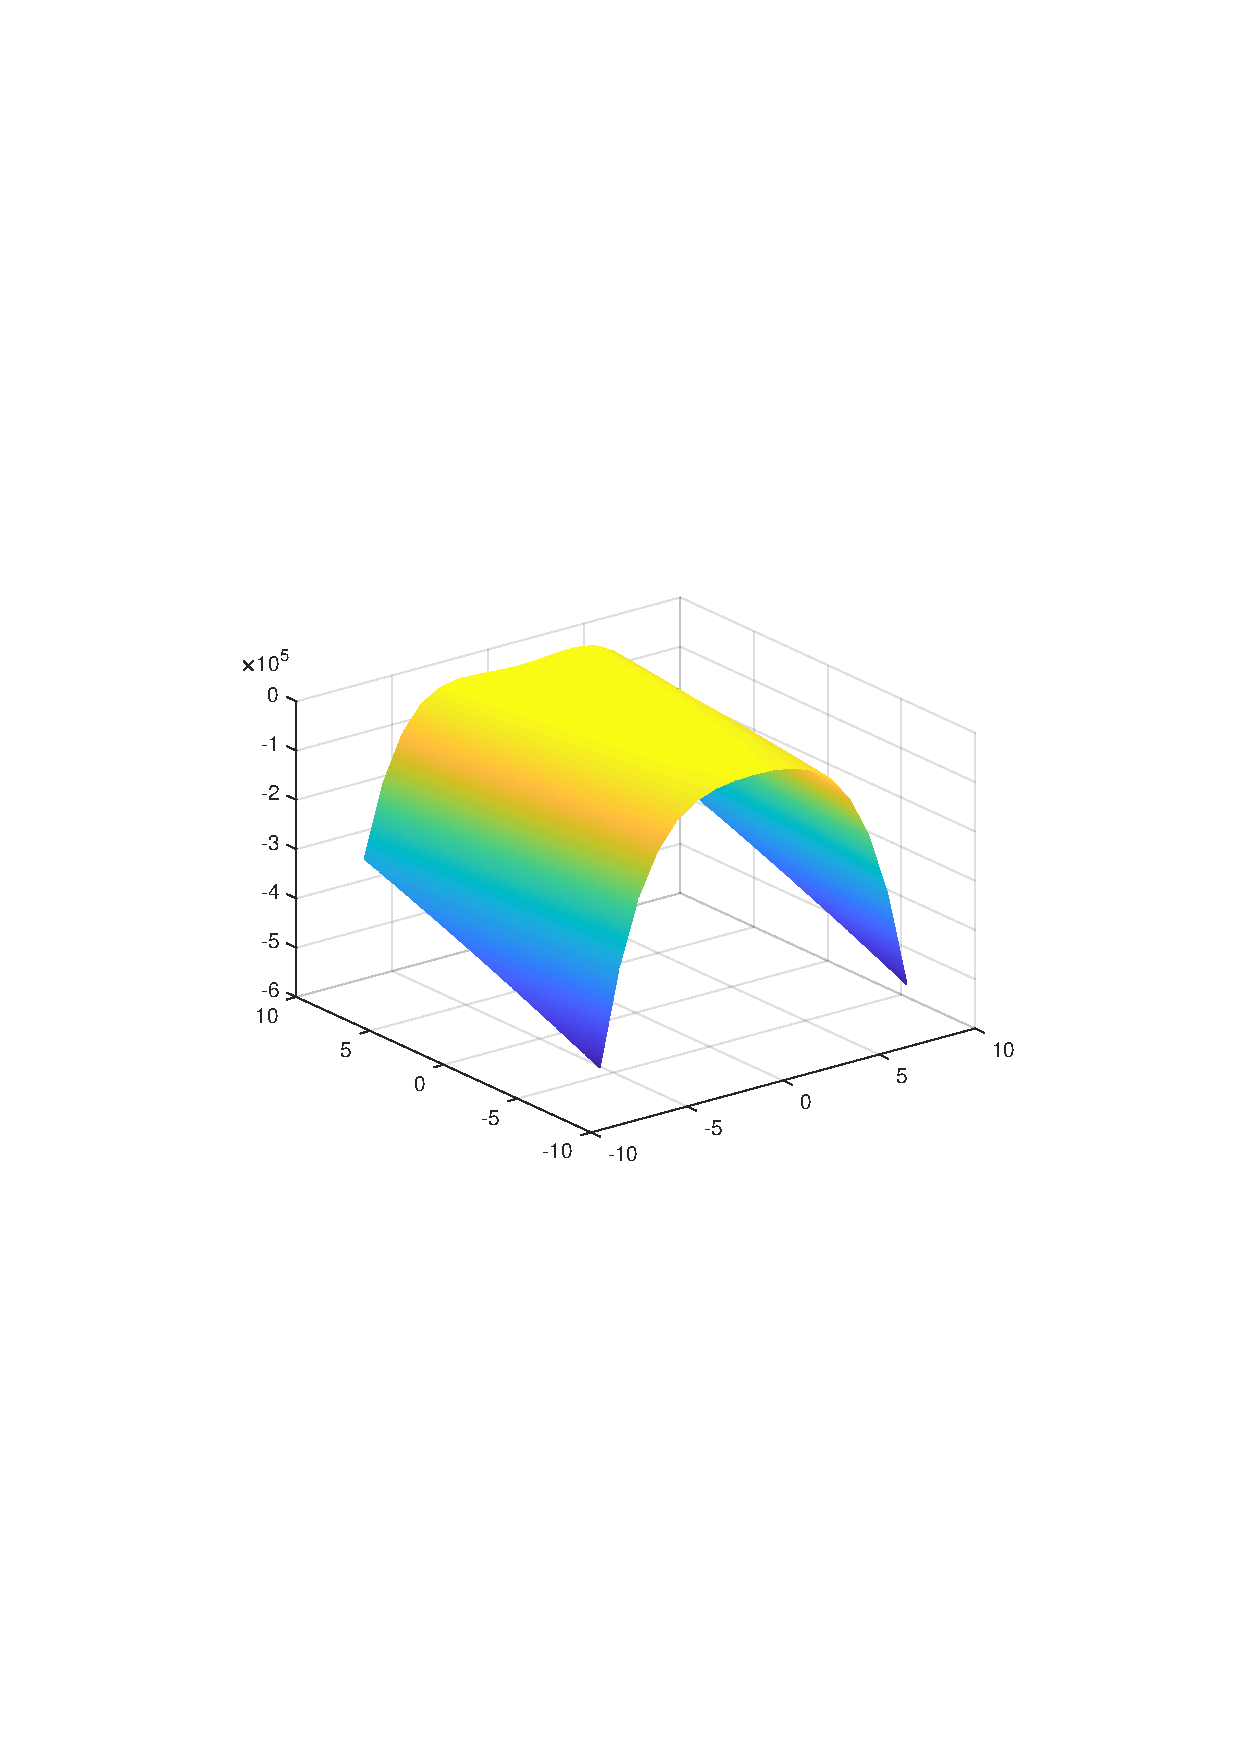
\includegraphics[width=12cm]{fig/0_1.pdf}
\caption{Rosenbrock函数图像}
\end{figure}

\begin{figure}[H]
\centering
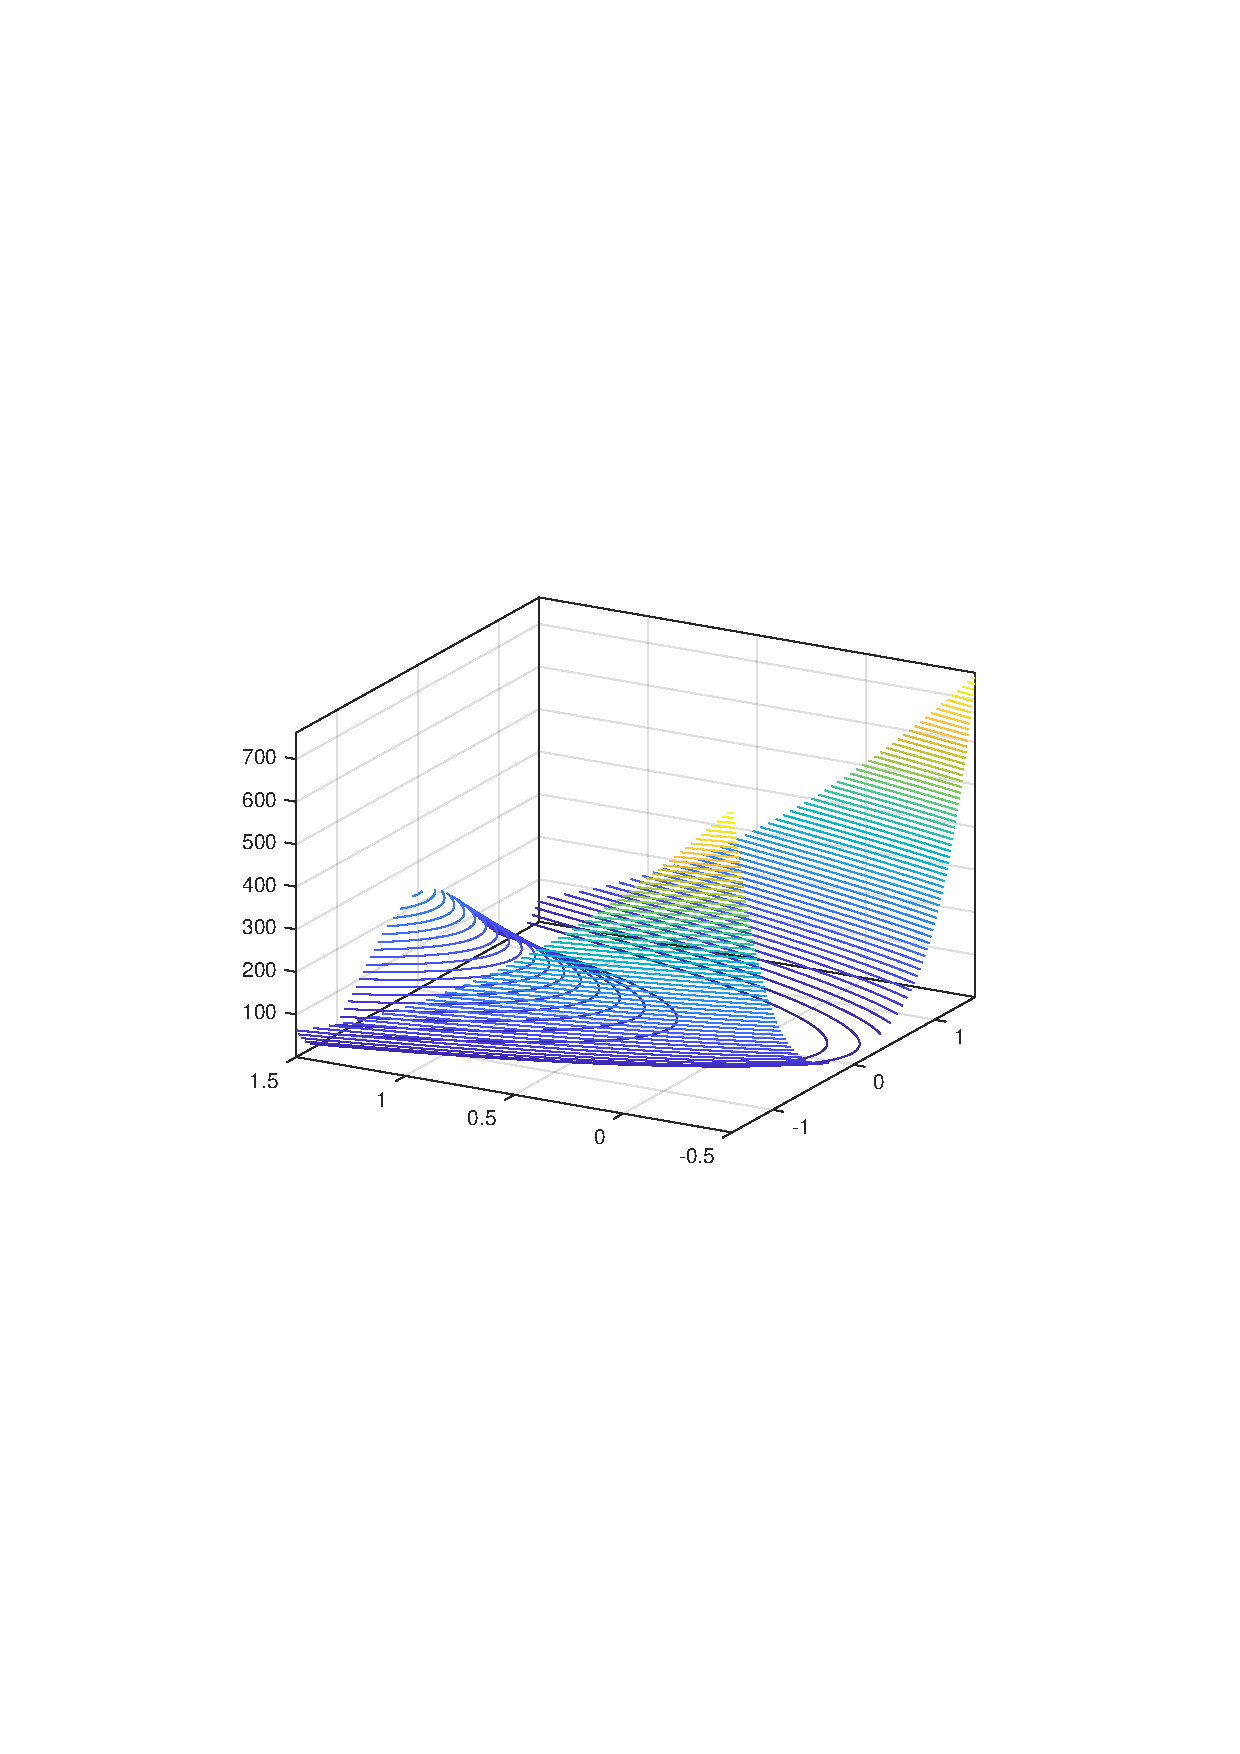
\includegraphics[width=12cm]{fig/0_2.pdf}
\caption{在$(1,1)$处附近的三维等高线}
\end{figure}

\begin{figure}[H]
\centering
\subfigure{
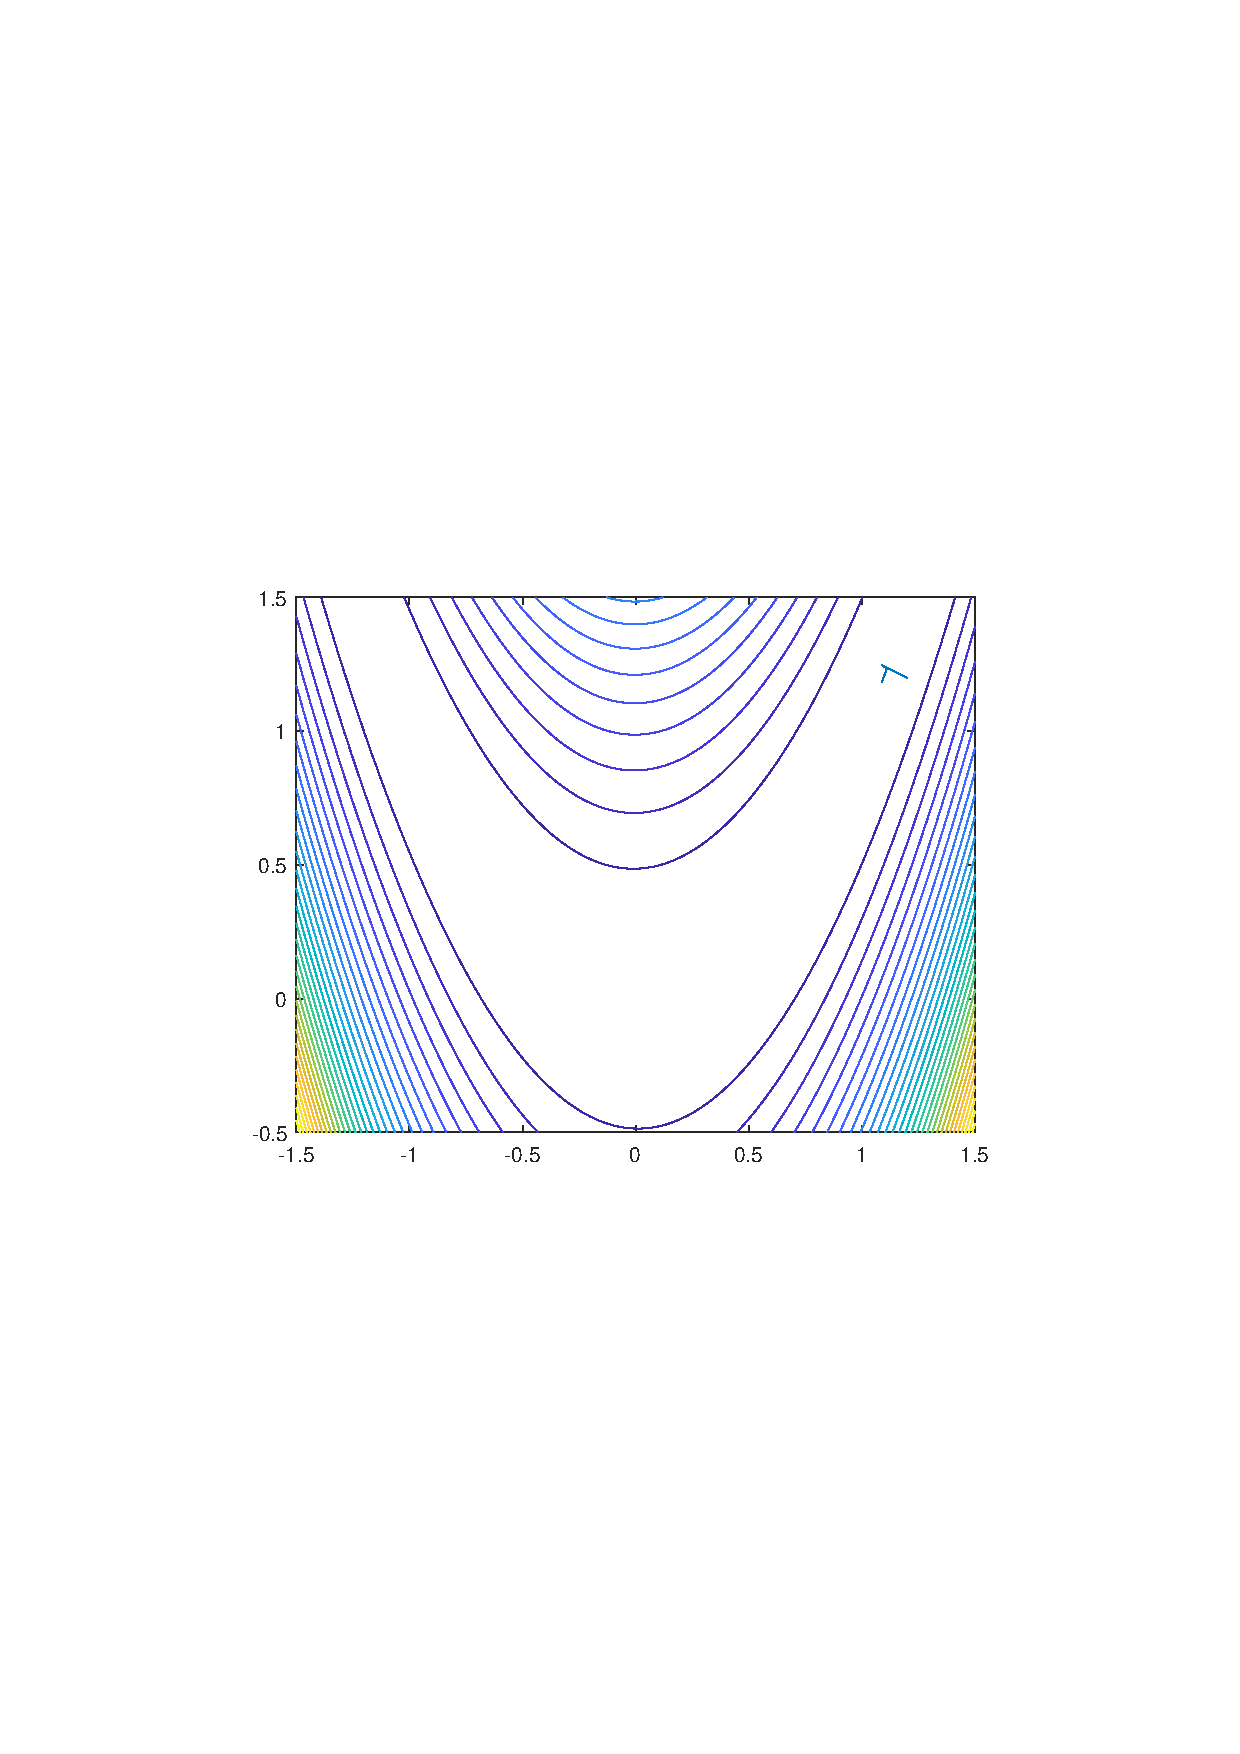
\includegraphics[width=5cm]{fig/1_1.pdf}}
\subfigure{
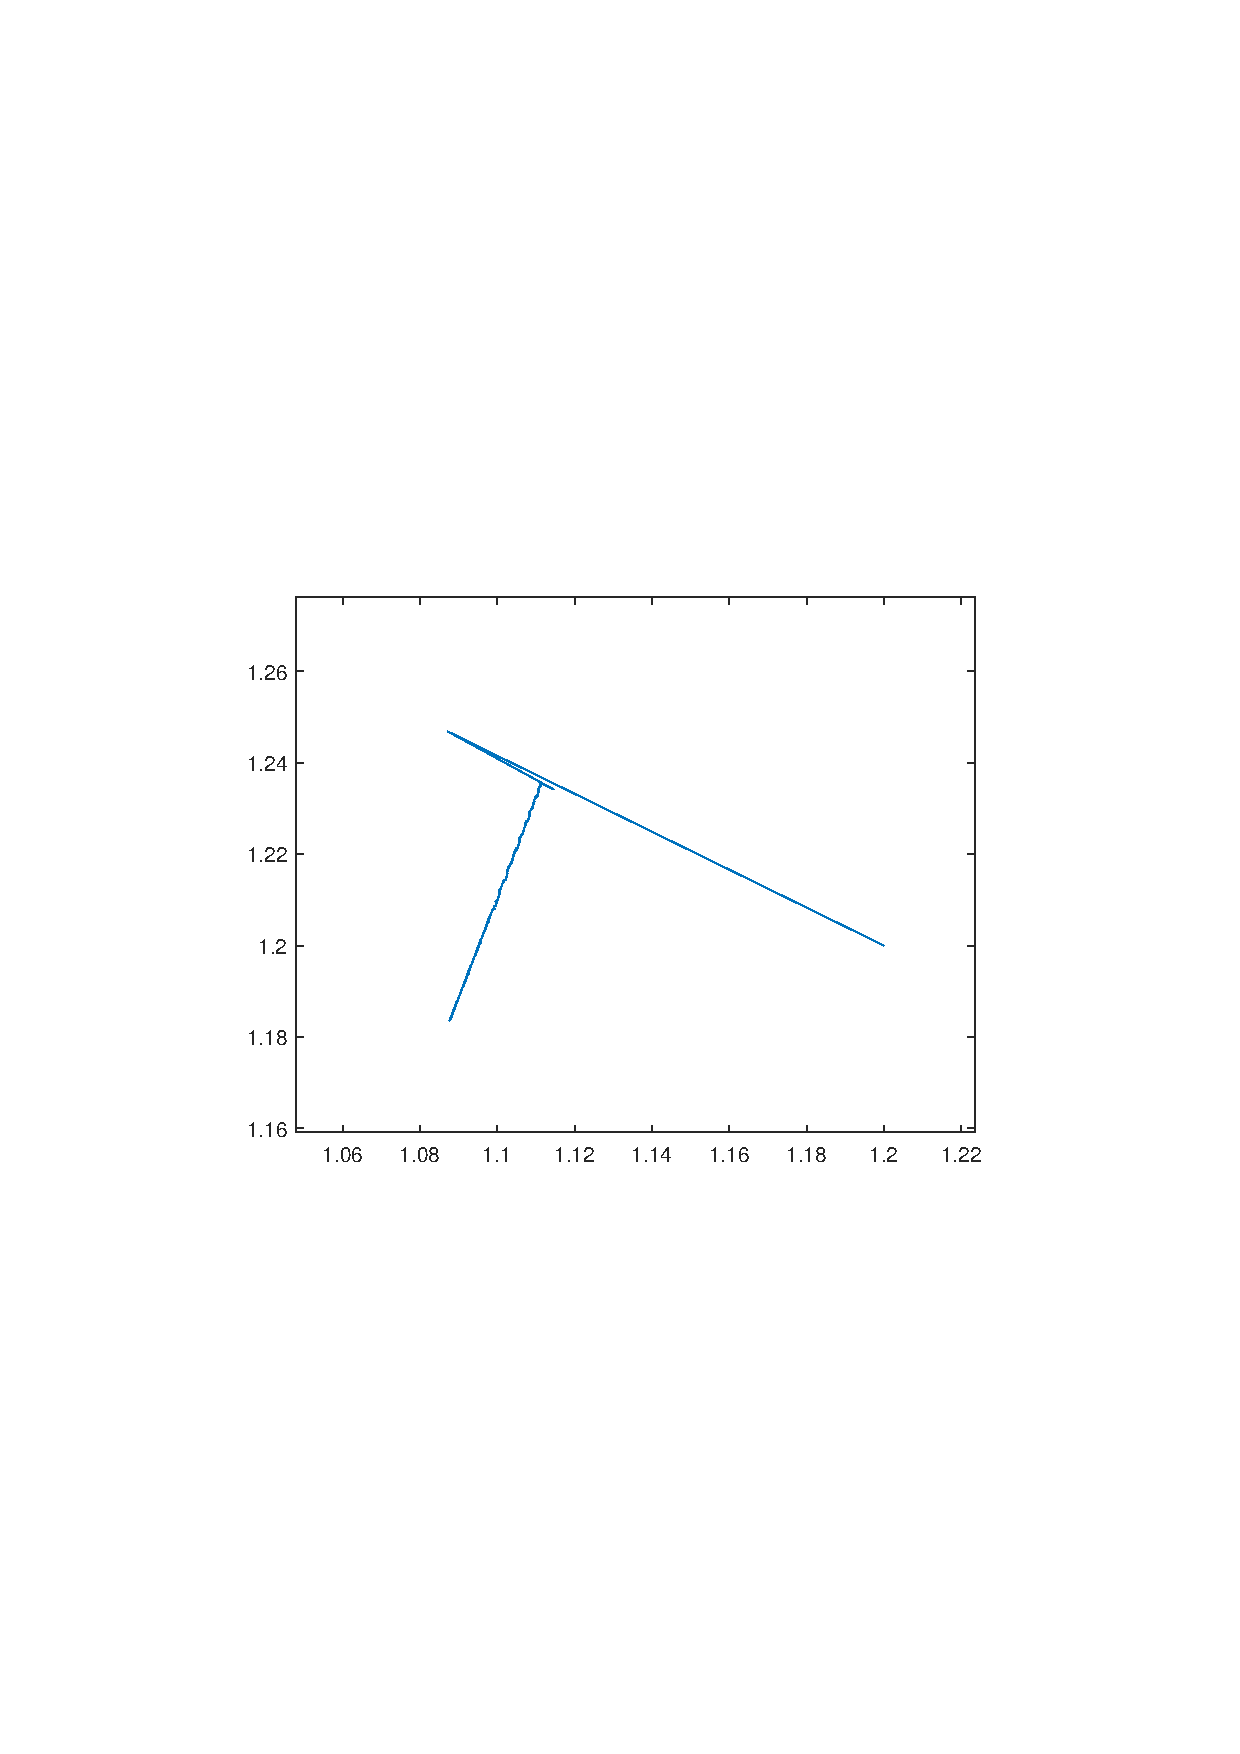
\includegraphics[width=5cm]{fig/1_2.pdf}}
\subfigure{
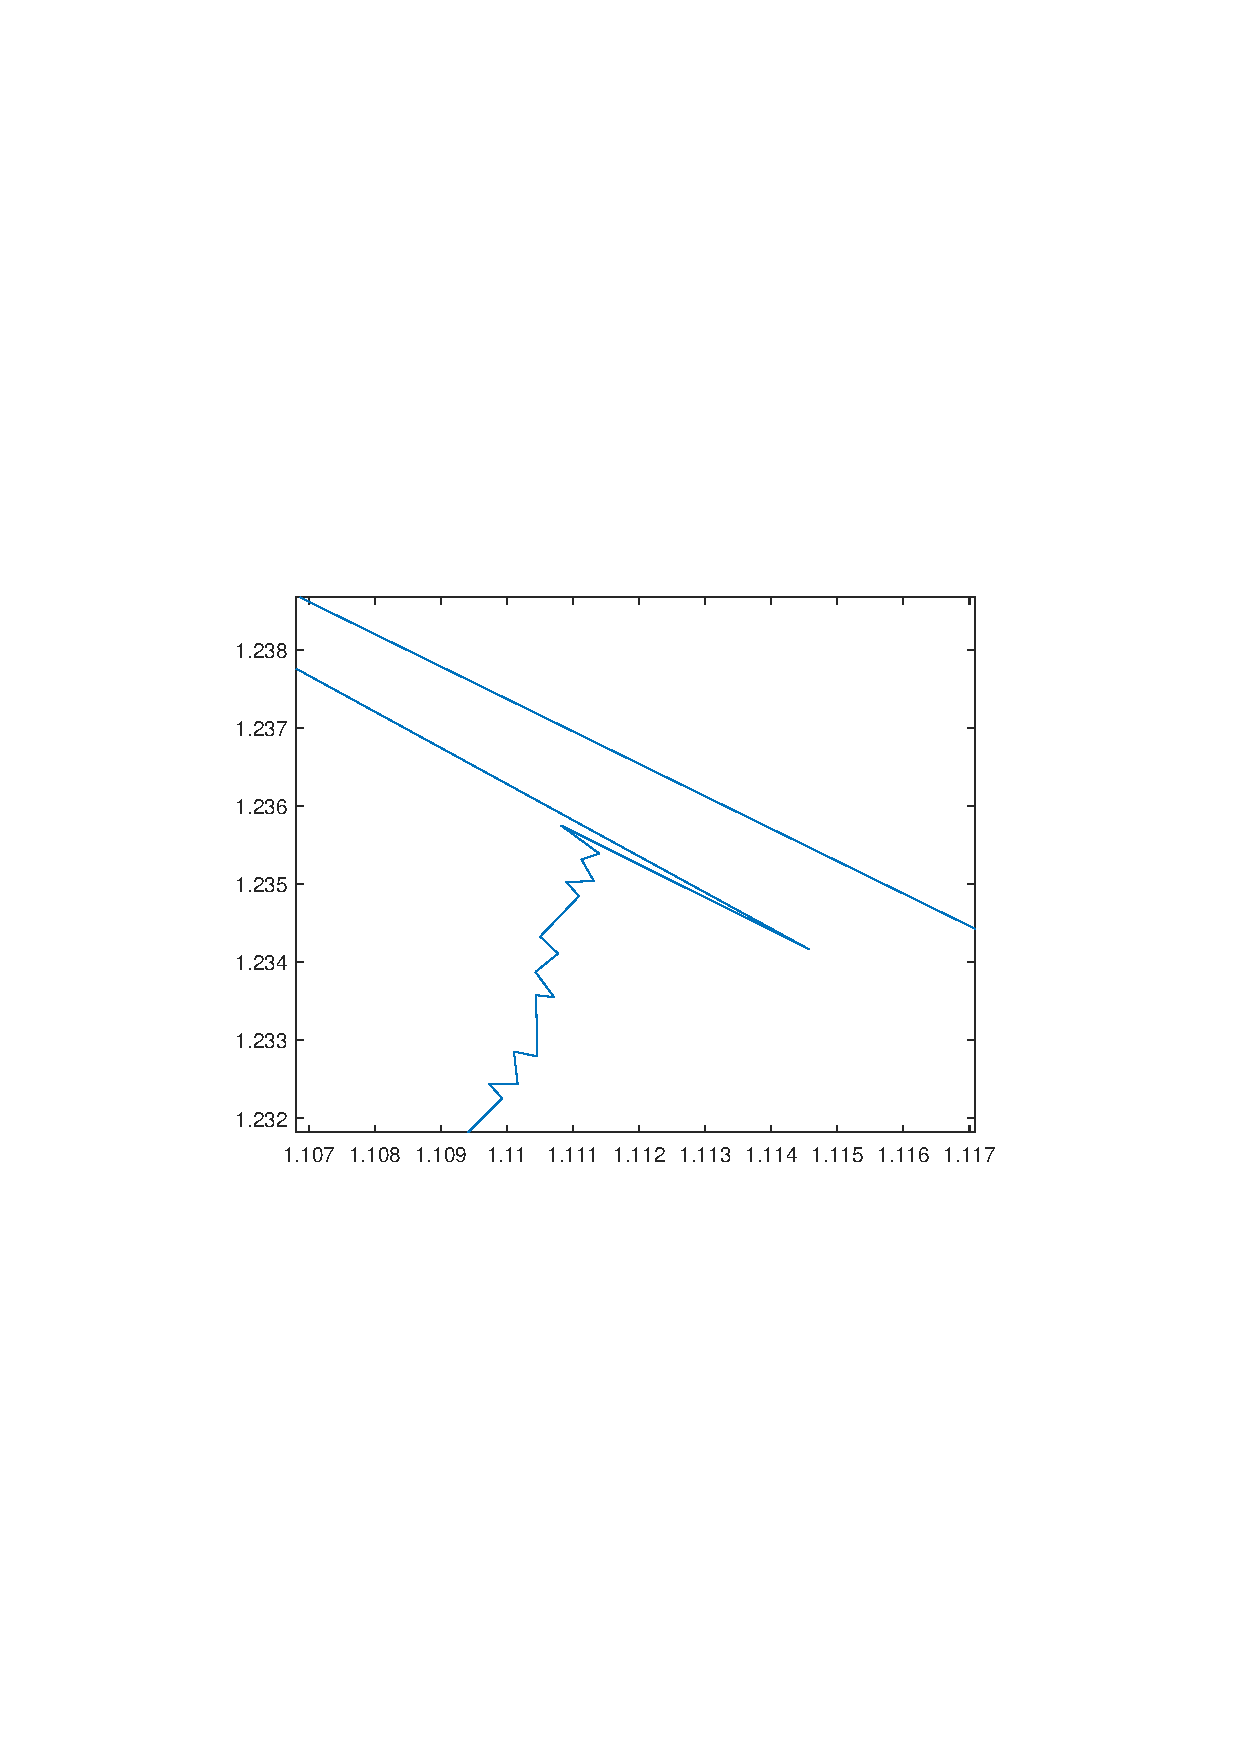
\includegraphics[width=5cm]{fig/1_3.pdf}}
\subfigure{
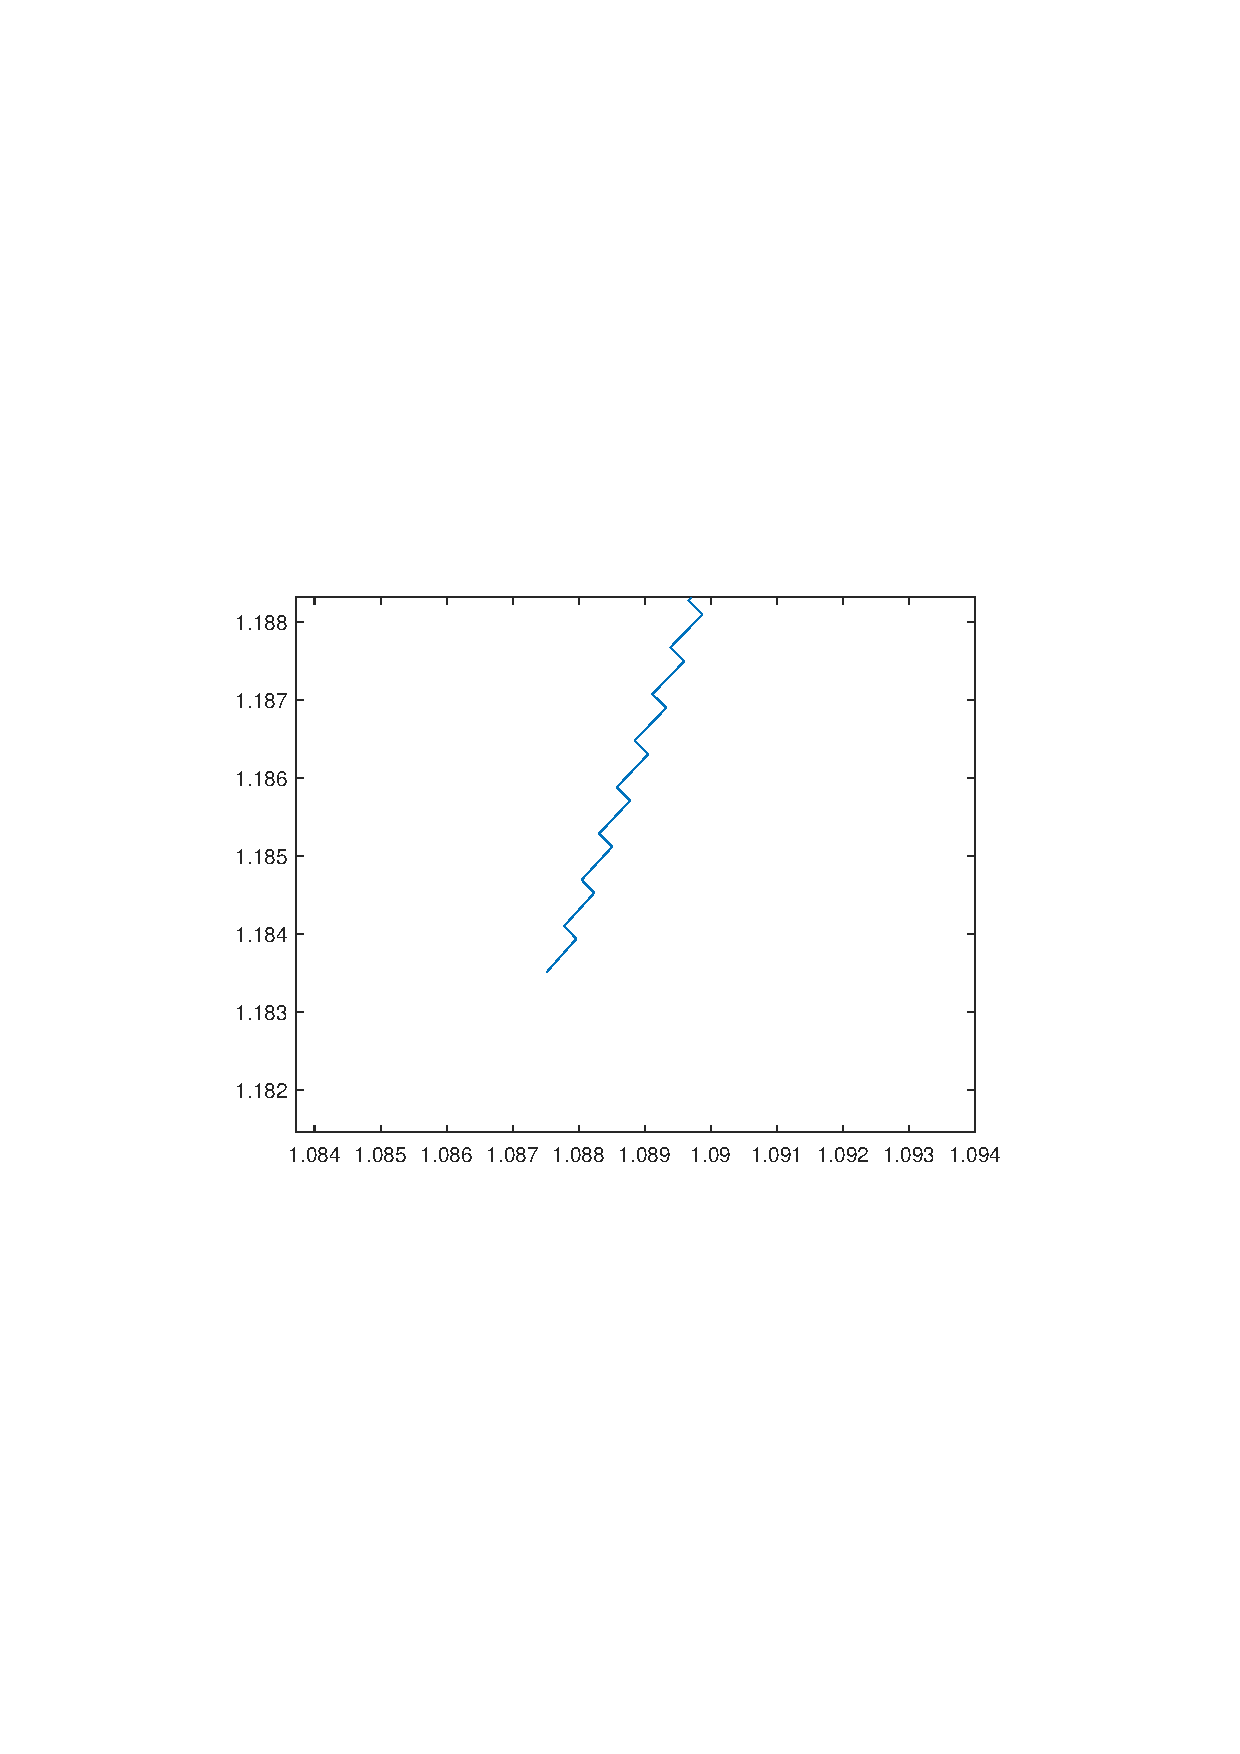
\includegraphics[width=5cm]{fig/1_4.pdf}}
\caption{Steepest-denscent in (1.2,1.2)}
\label{Fig.lable}
\end{figure}

\begin{figure}[H]
\centering
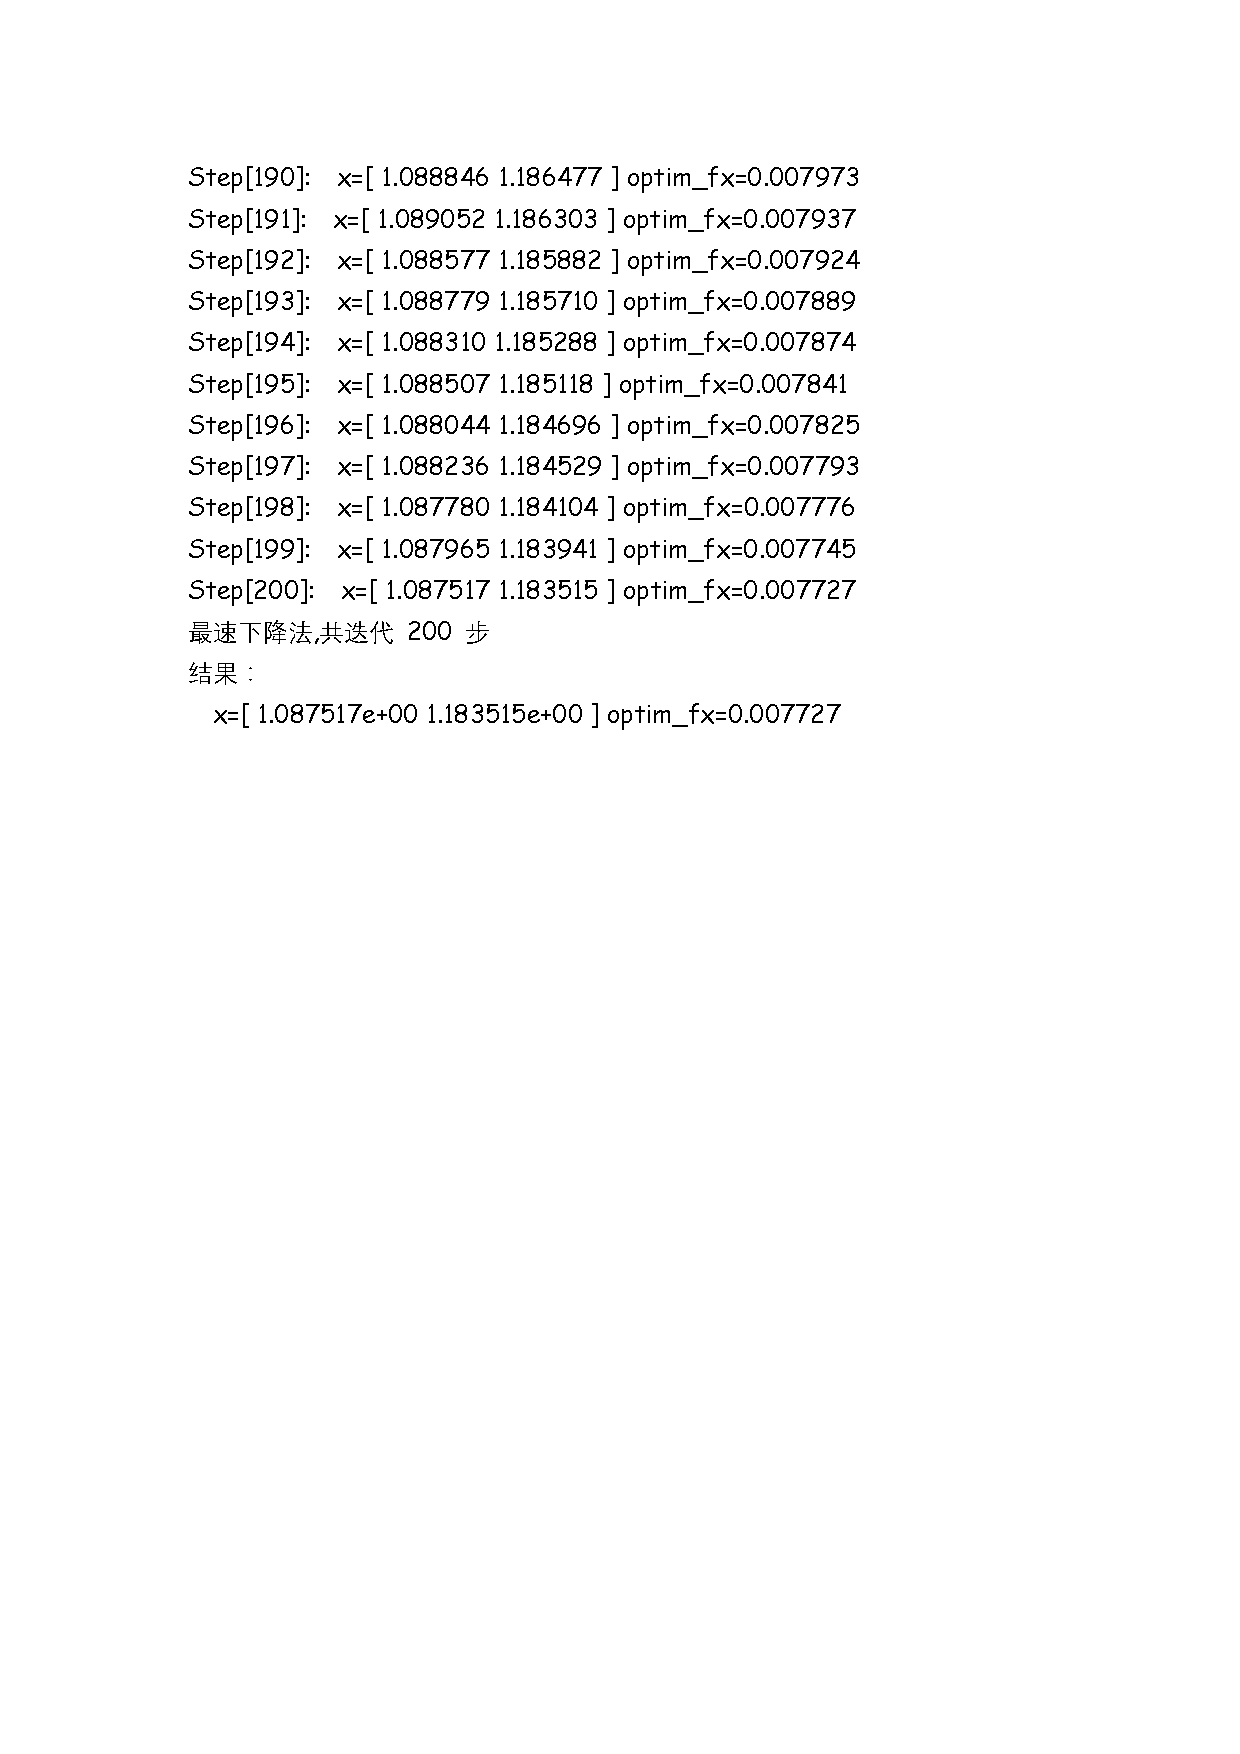
\includegraphics[width=10cm]{fig/1_5.pdf}
%\caption{在$(1,1)$处附近的三维等高线}
\end{figure}

\begin{figure}[H]
\centering
\subfigure{
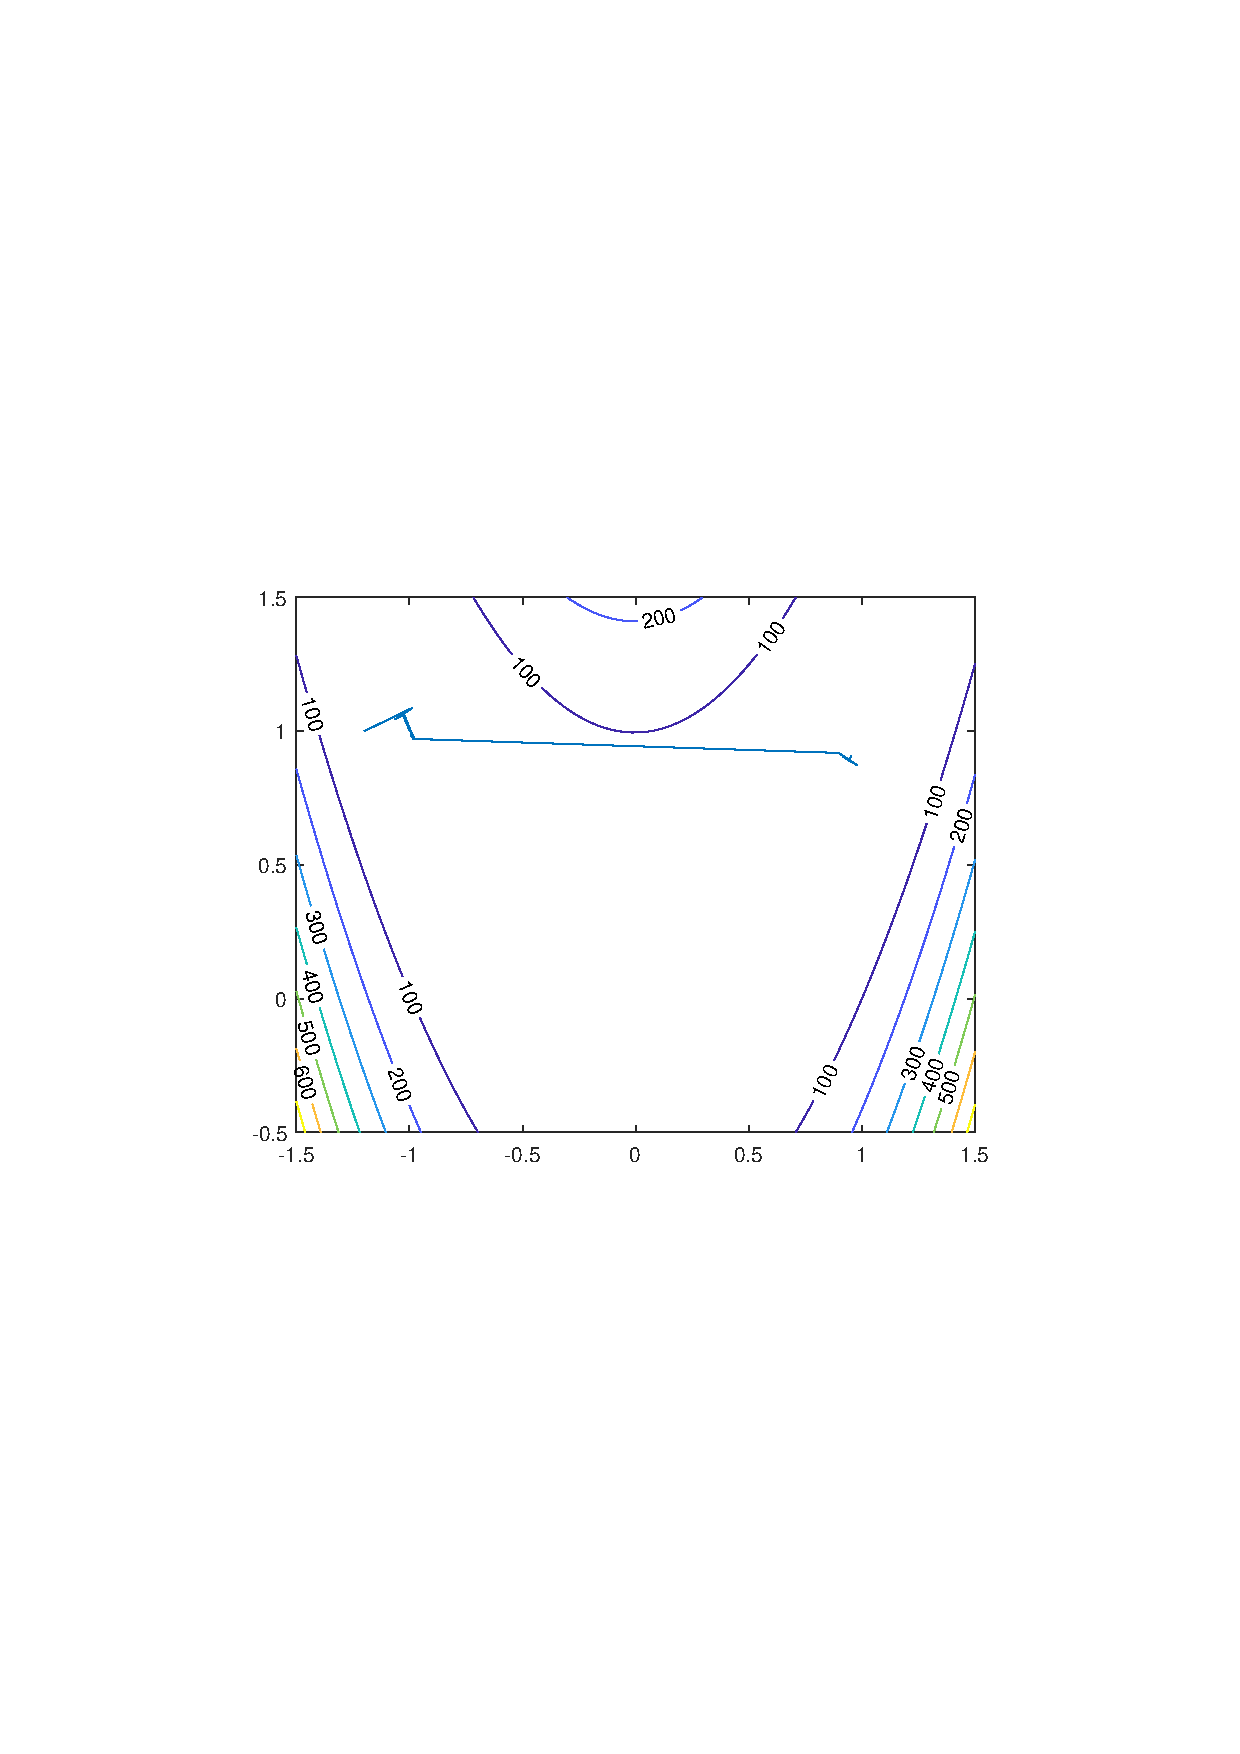
\includegraphics[width=5cm]{fig/2_1.pdf}}
\subfigure{
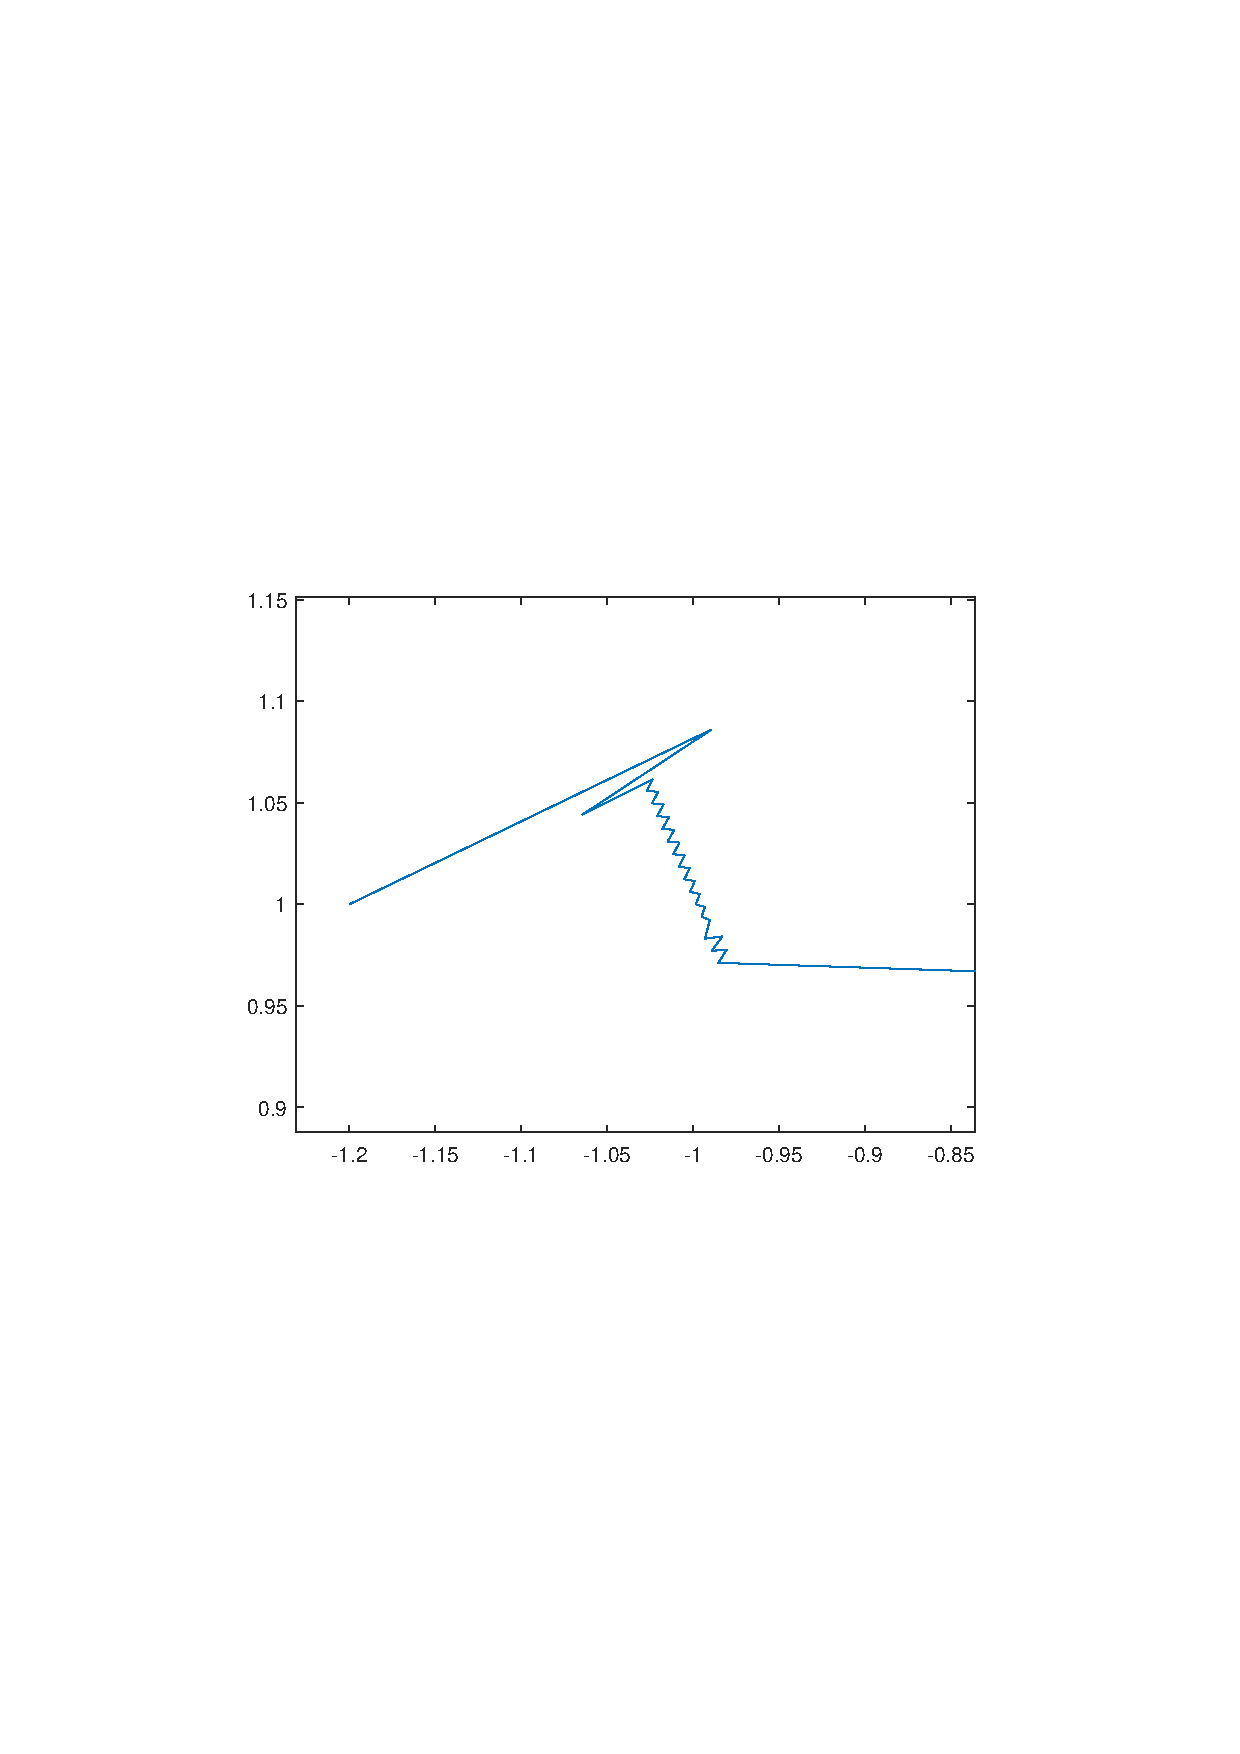
\includegraphics[width=5cm]{fig/2_2.pdf}}
\subfigure{
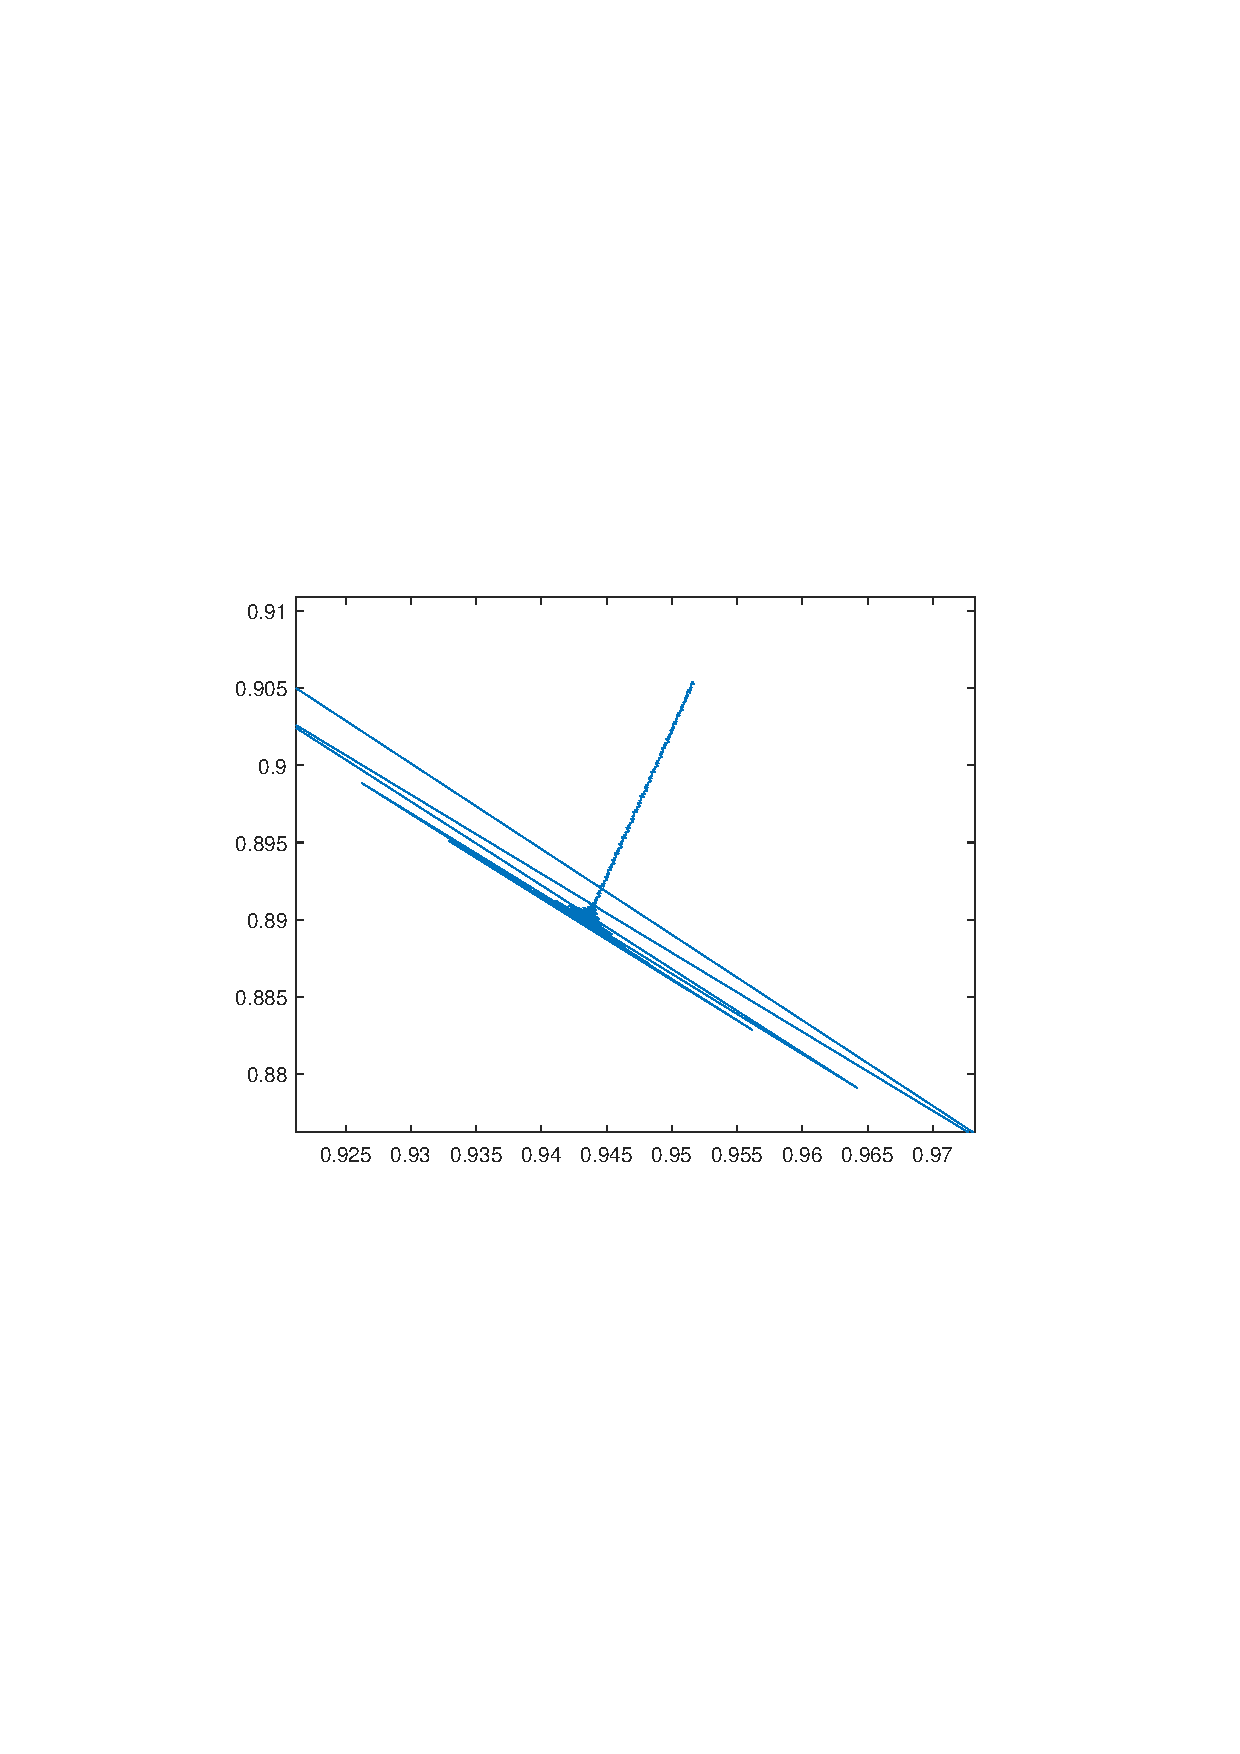
\includegraphics[width=5cm]{fig/2_3.pdf}}
\subfigure{
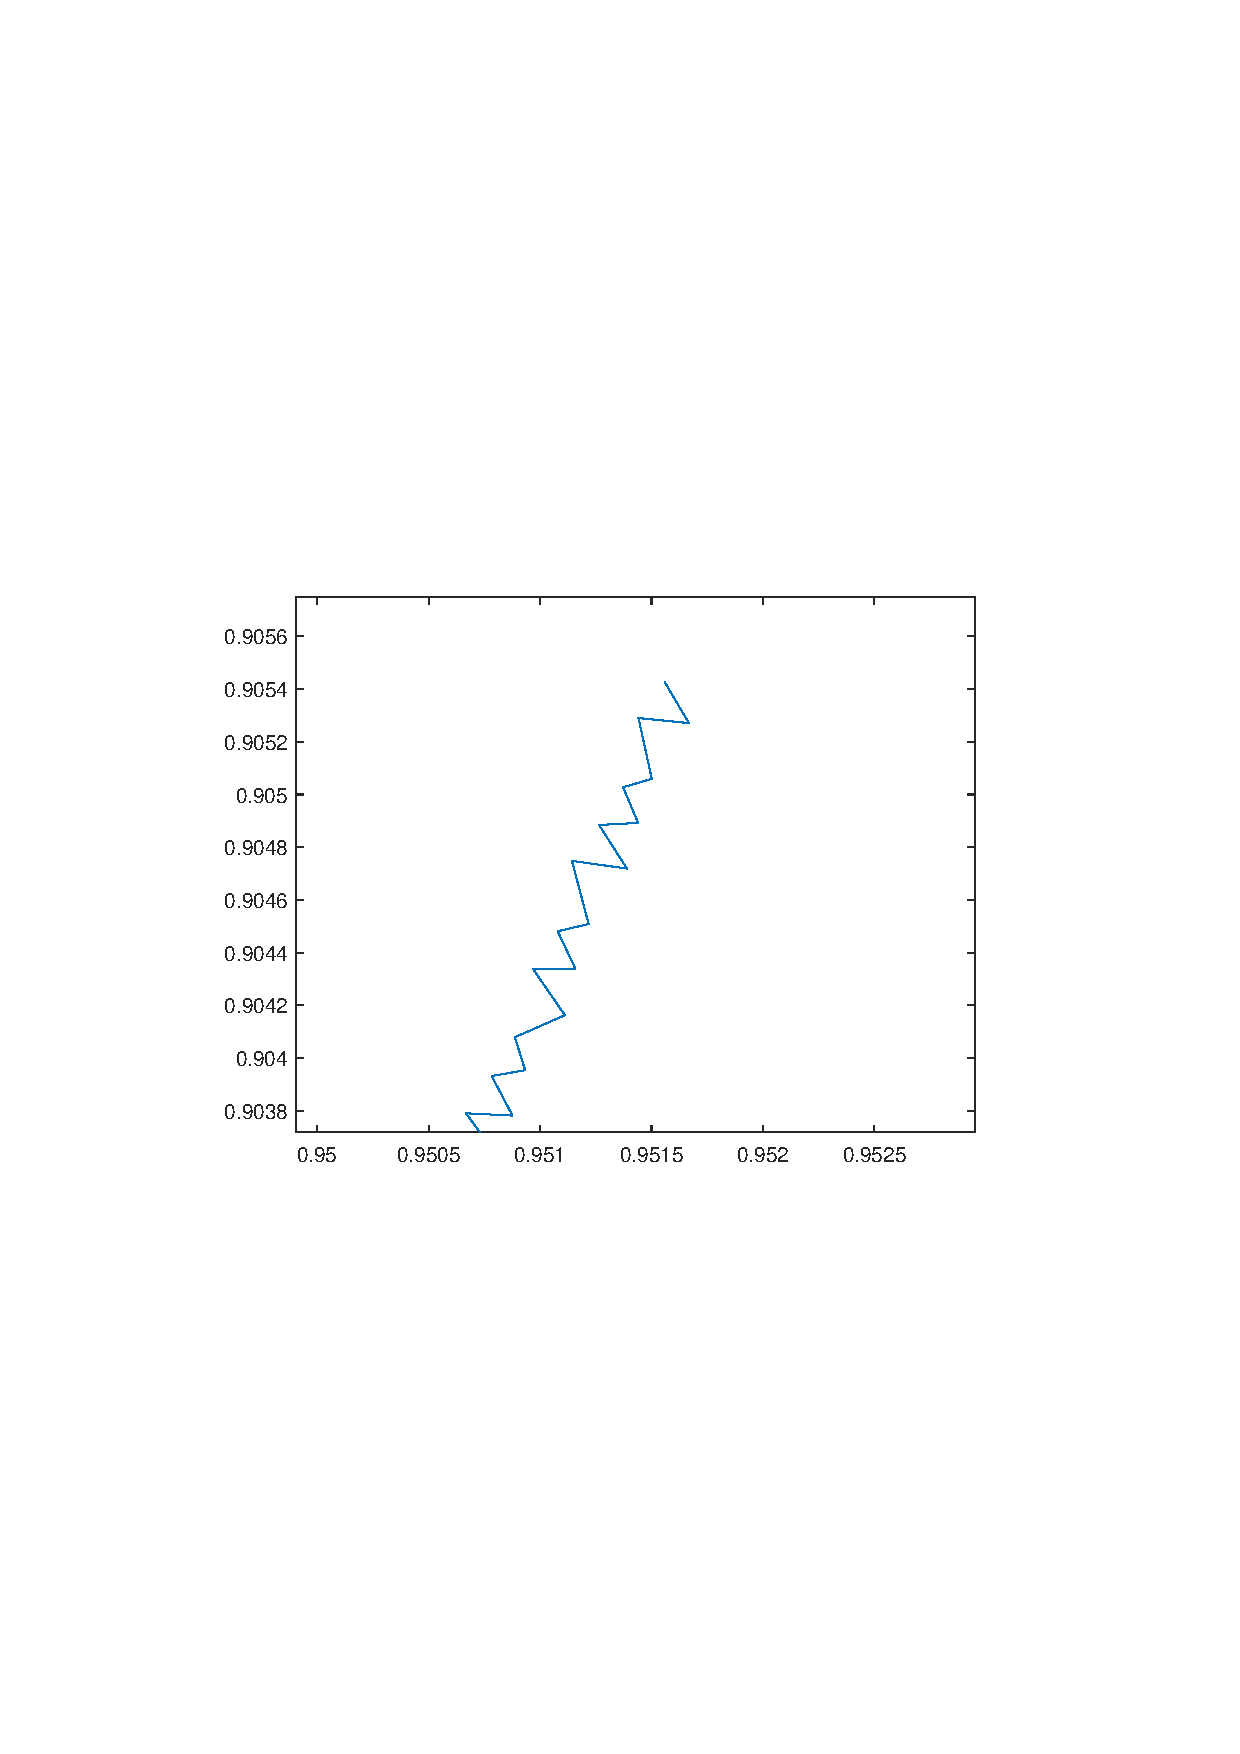
\includegraphics[width=5cm]{fig/2_4.pdf}}
\caption{Steepest-denscent in (-1.2,1)}
\label{Fig.lable}
\end{figure}

\begin{figure}[H]
\centering
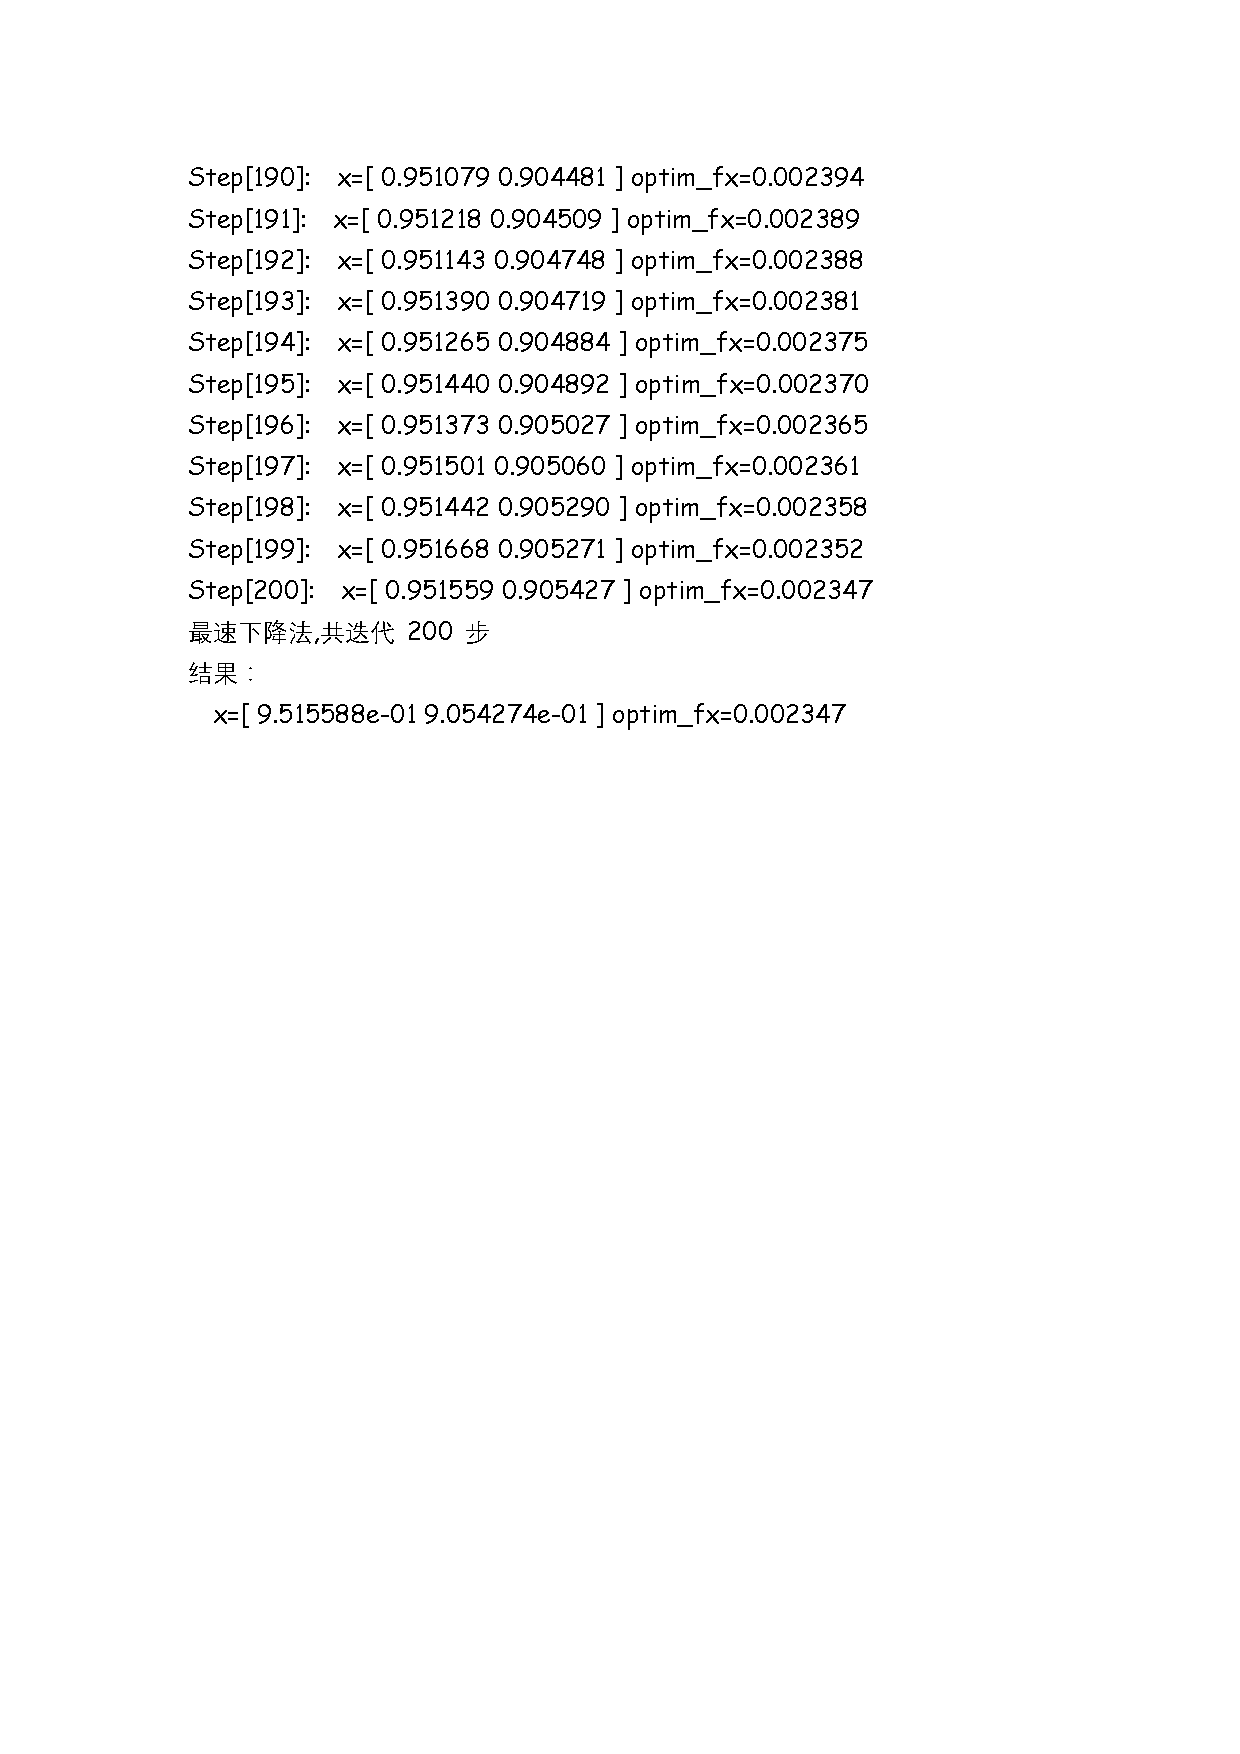
\includegraphics[width=10cm]{fig/2_5.pdf}
%\caption{在$(1,1)$处附近的三维等高线}
\end{figure}

\begin{figure}[H]
\centering
\subfigure{
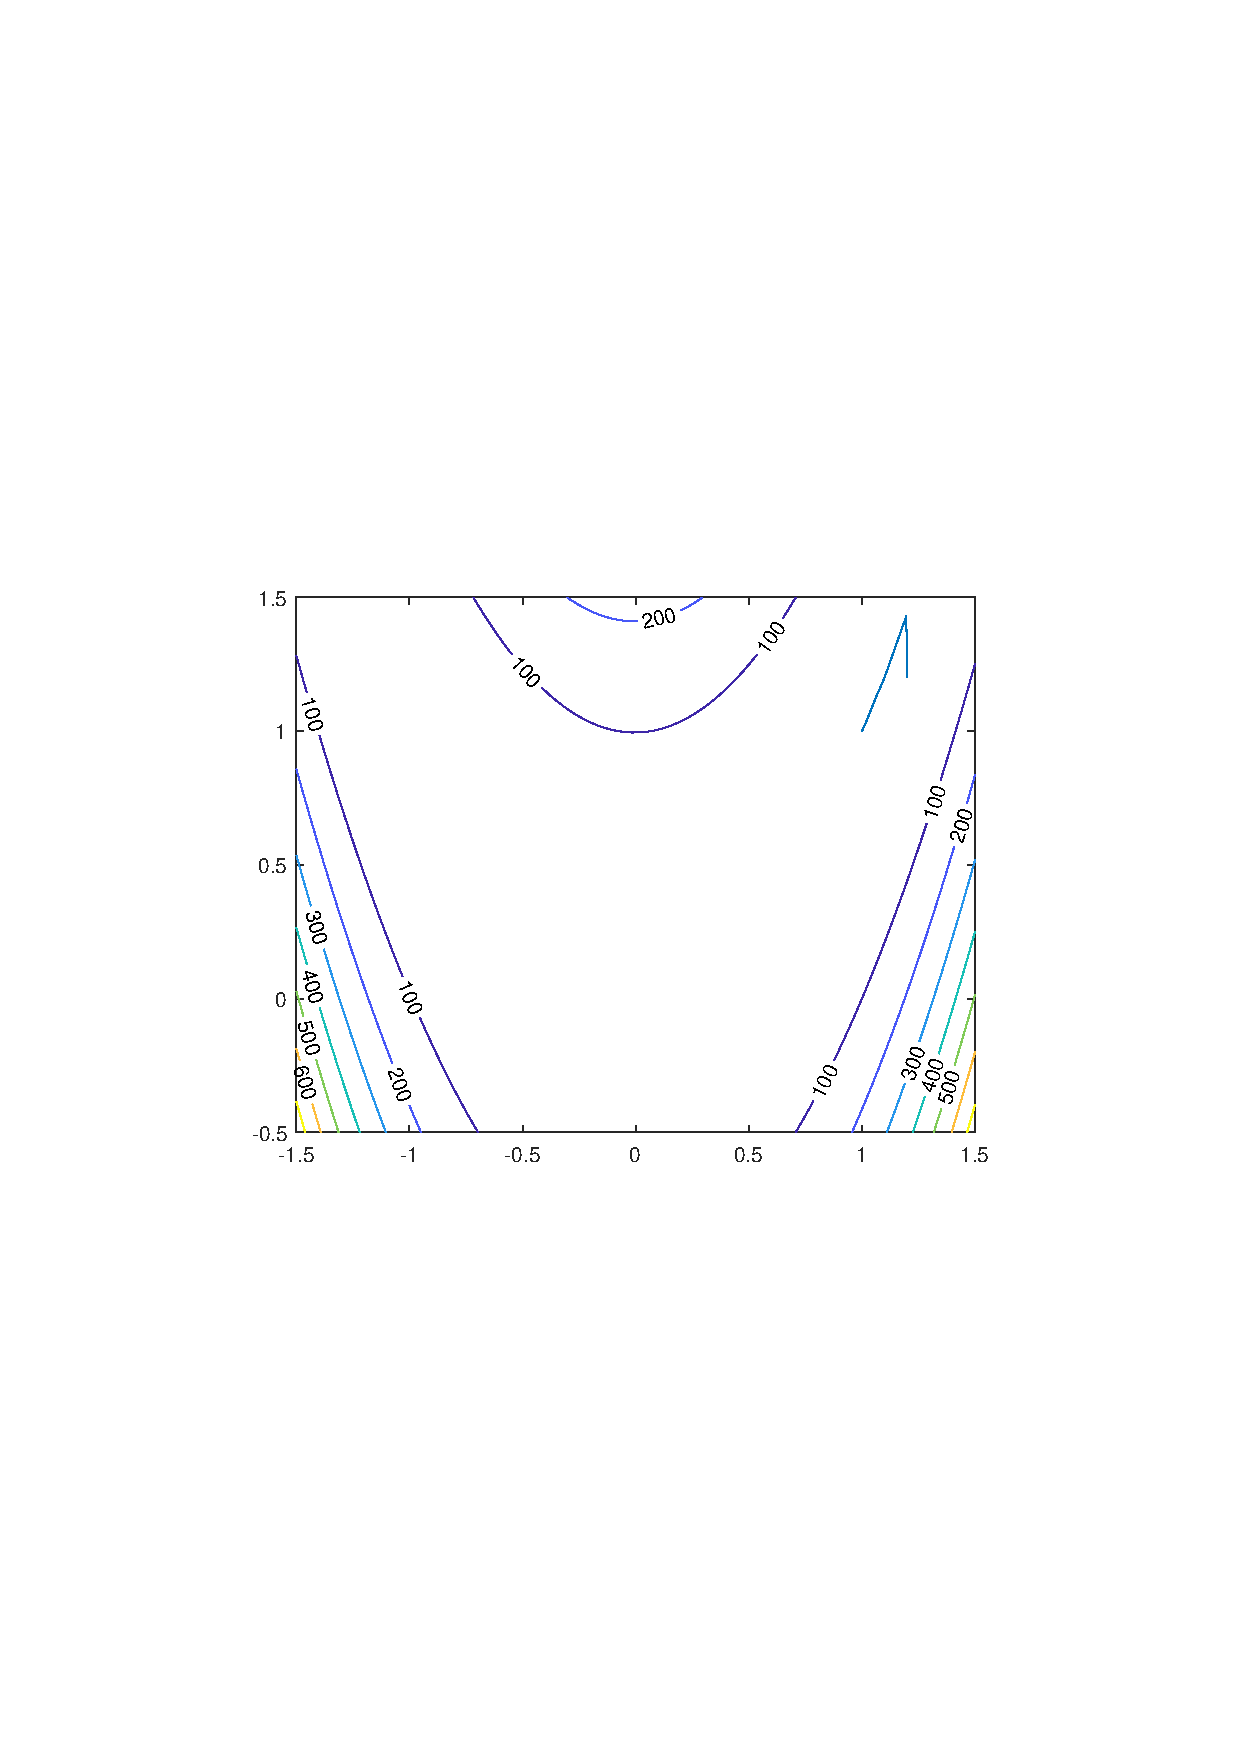
\includegraphics[width=5cm]{fig/3_1.pdf}}
\subfigure{
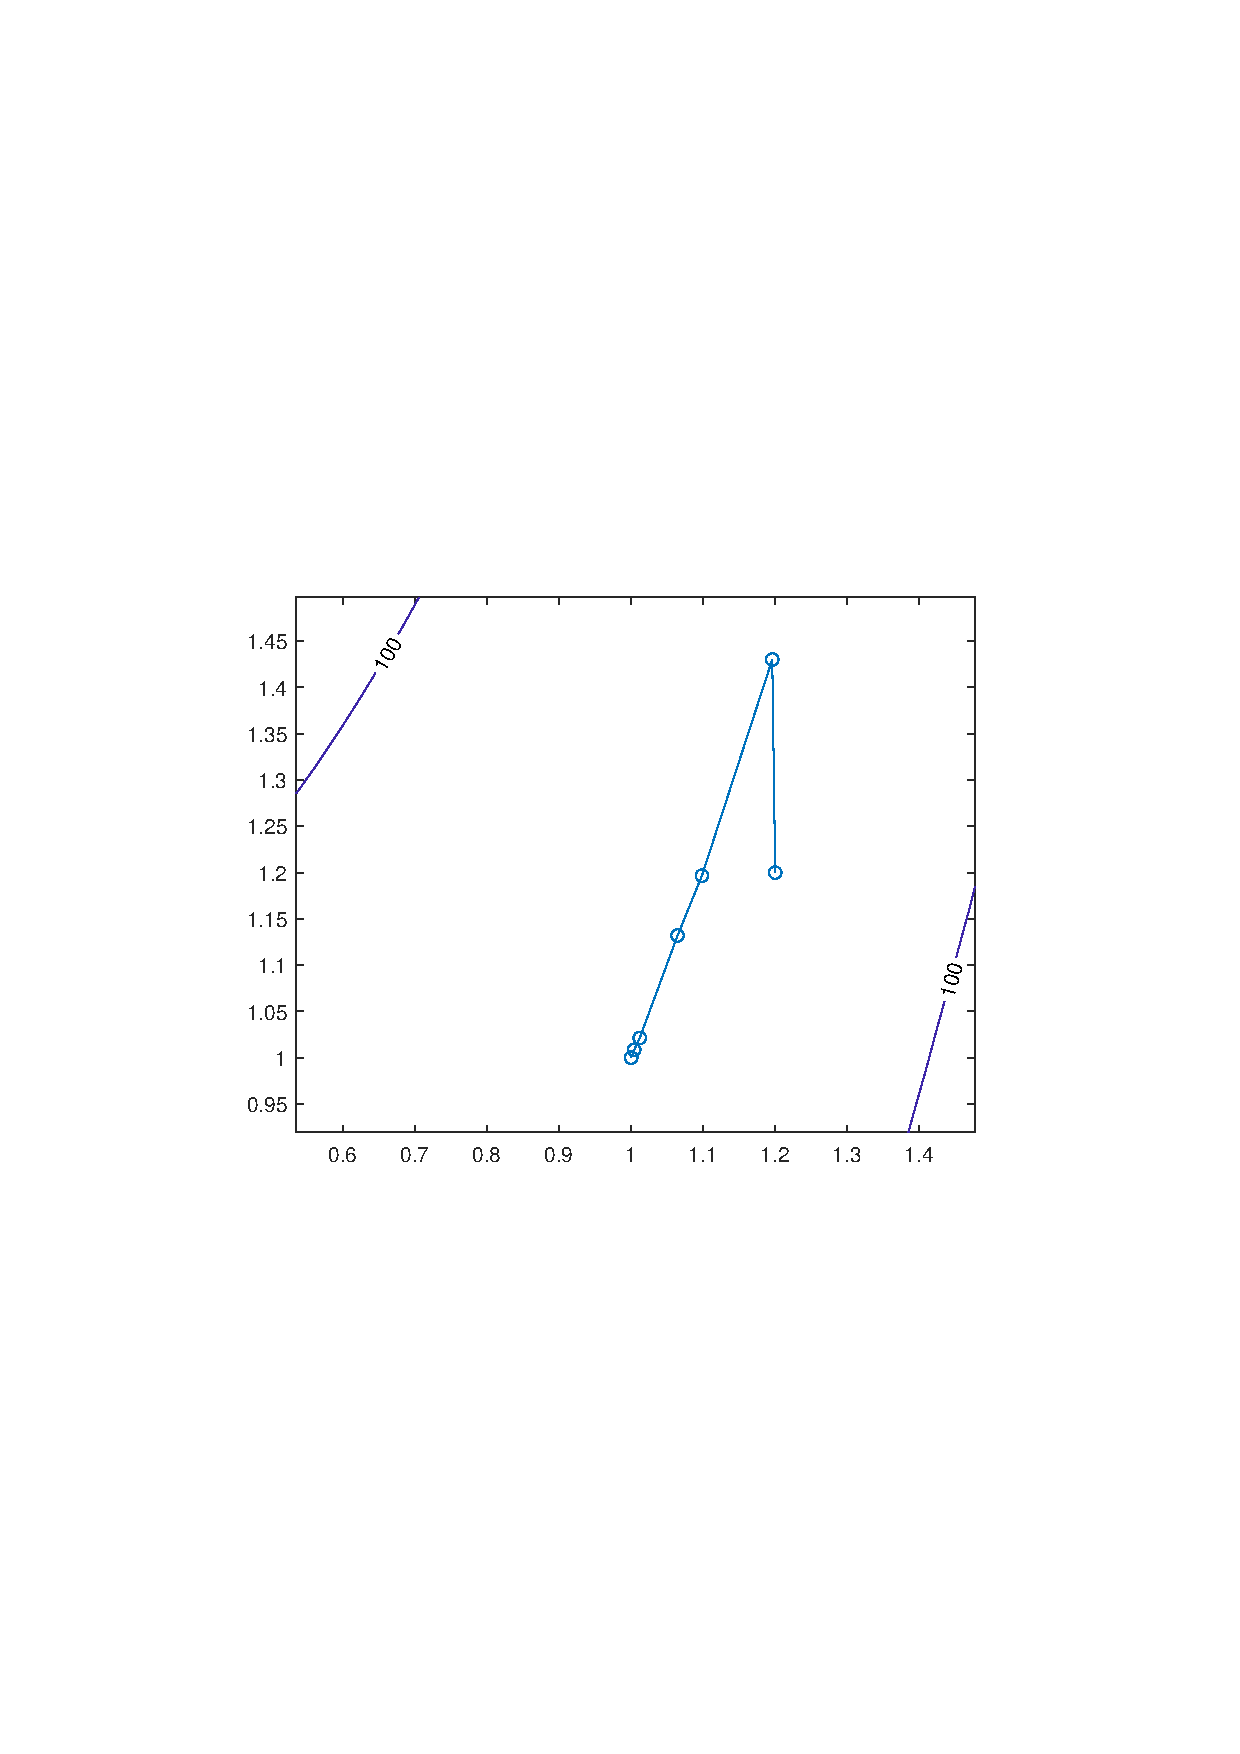
\includegraphics[width=5cm]{fig/3_2.pdf}}
\subfigure{
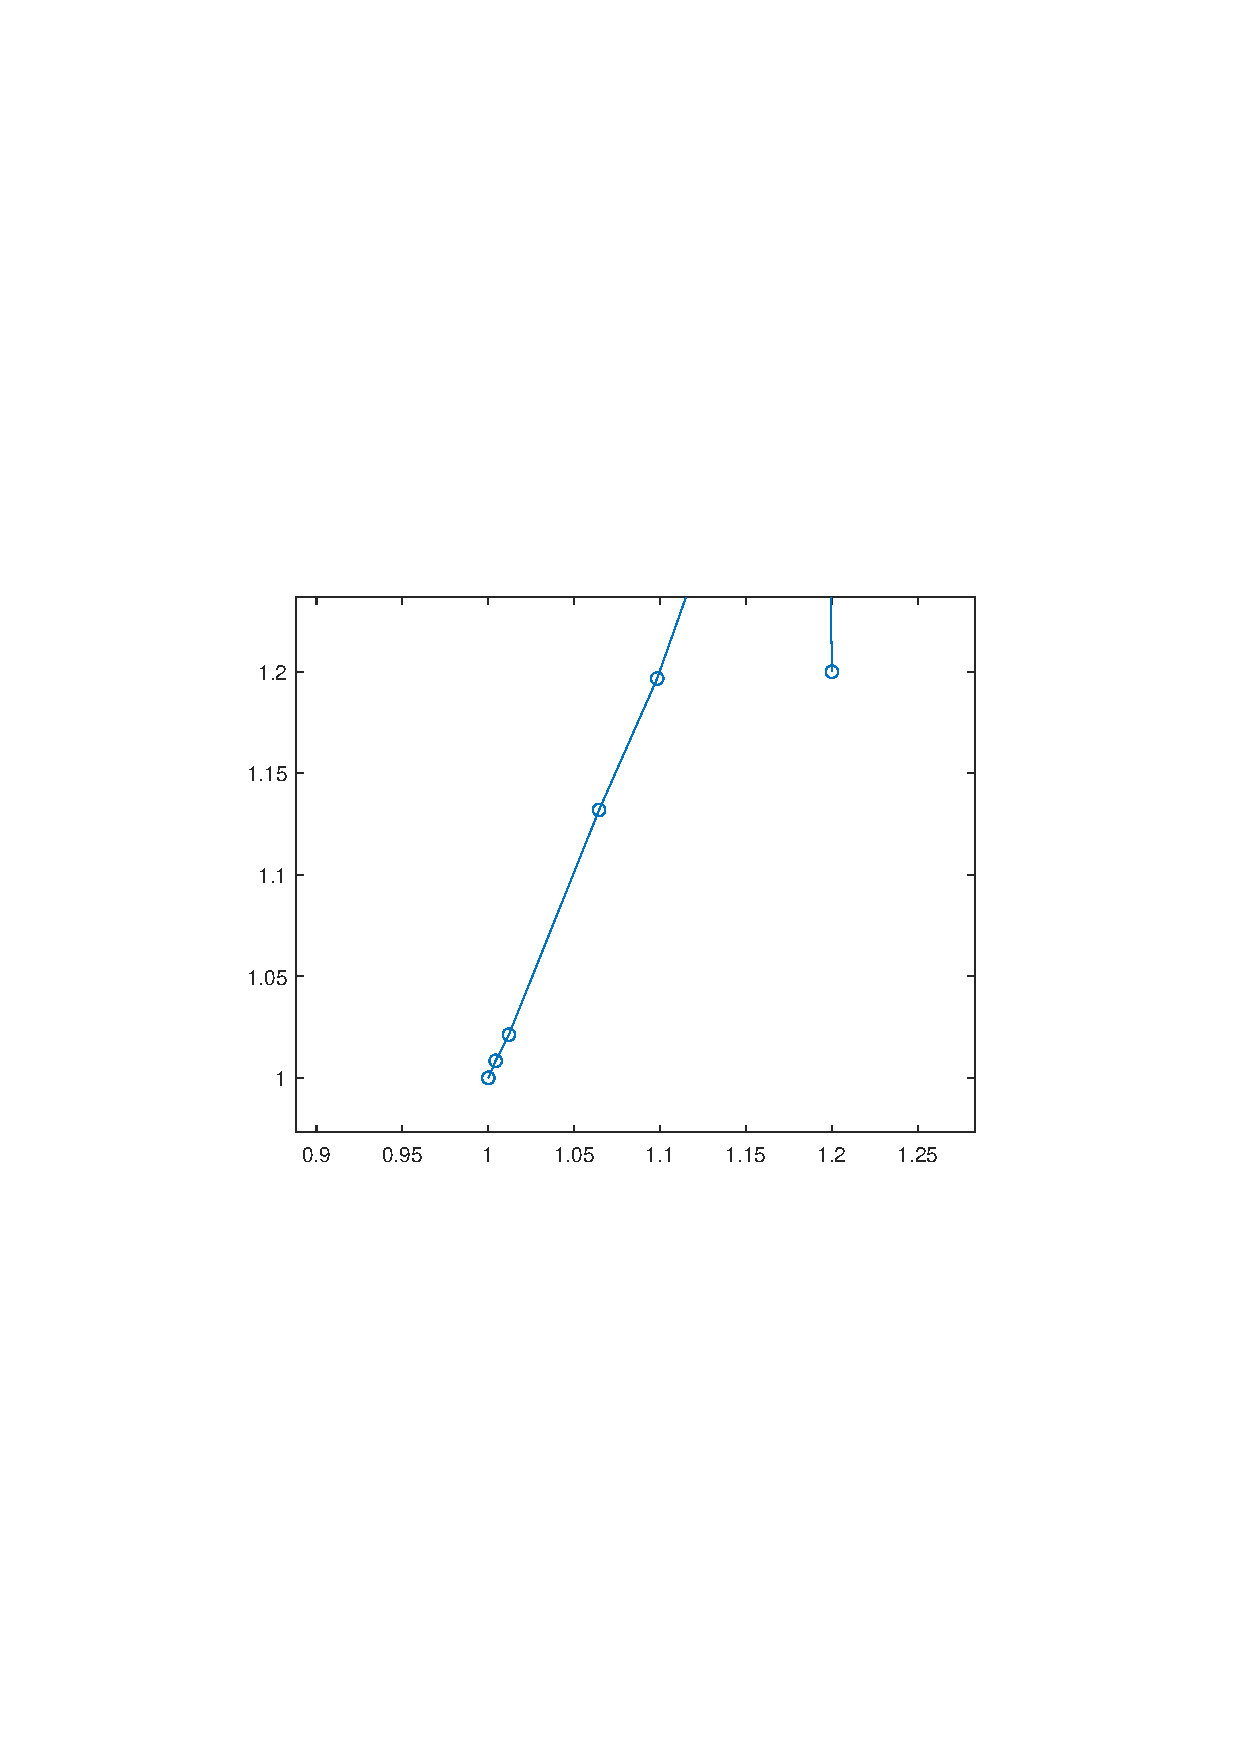
\includegraphics[width=5cm]{fig/3_3.pdf}}
\subfigure{
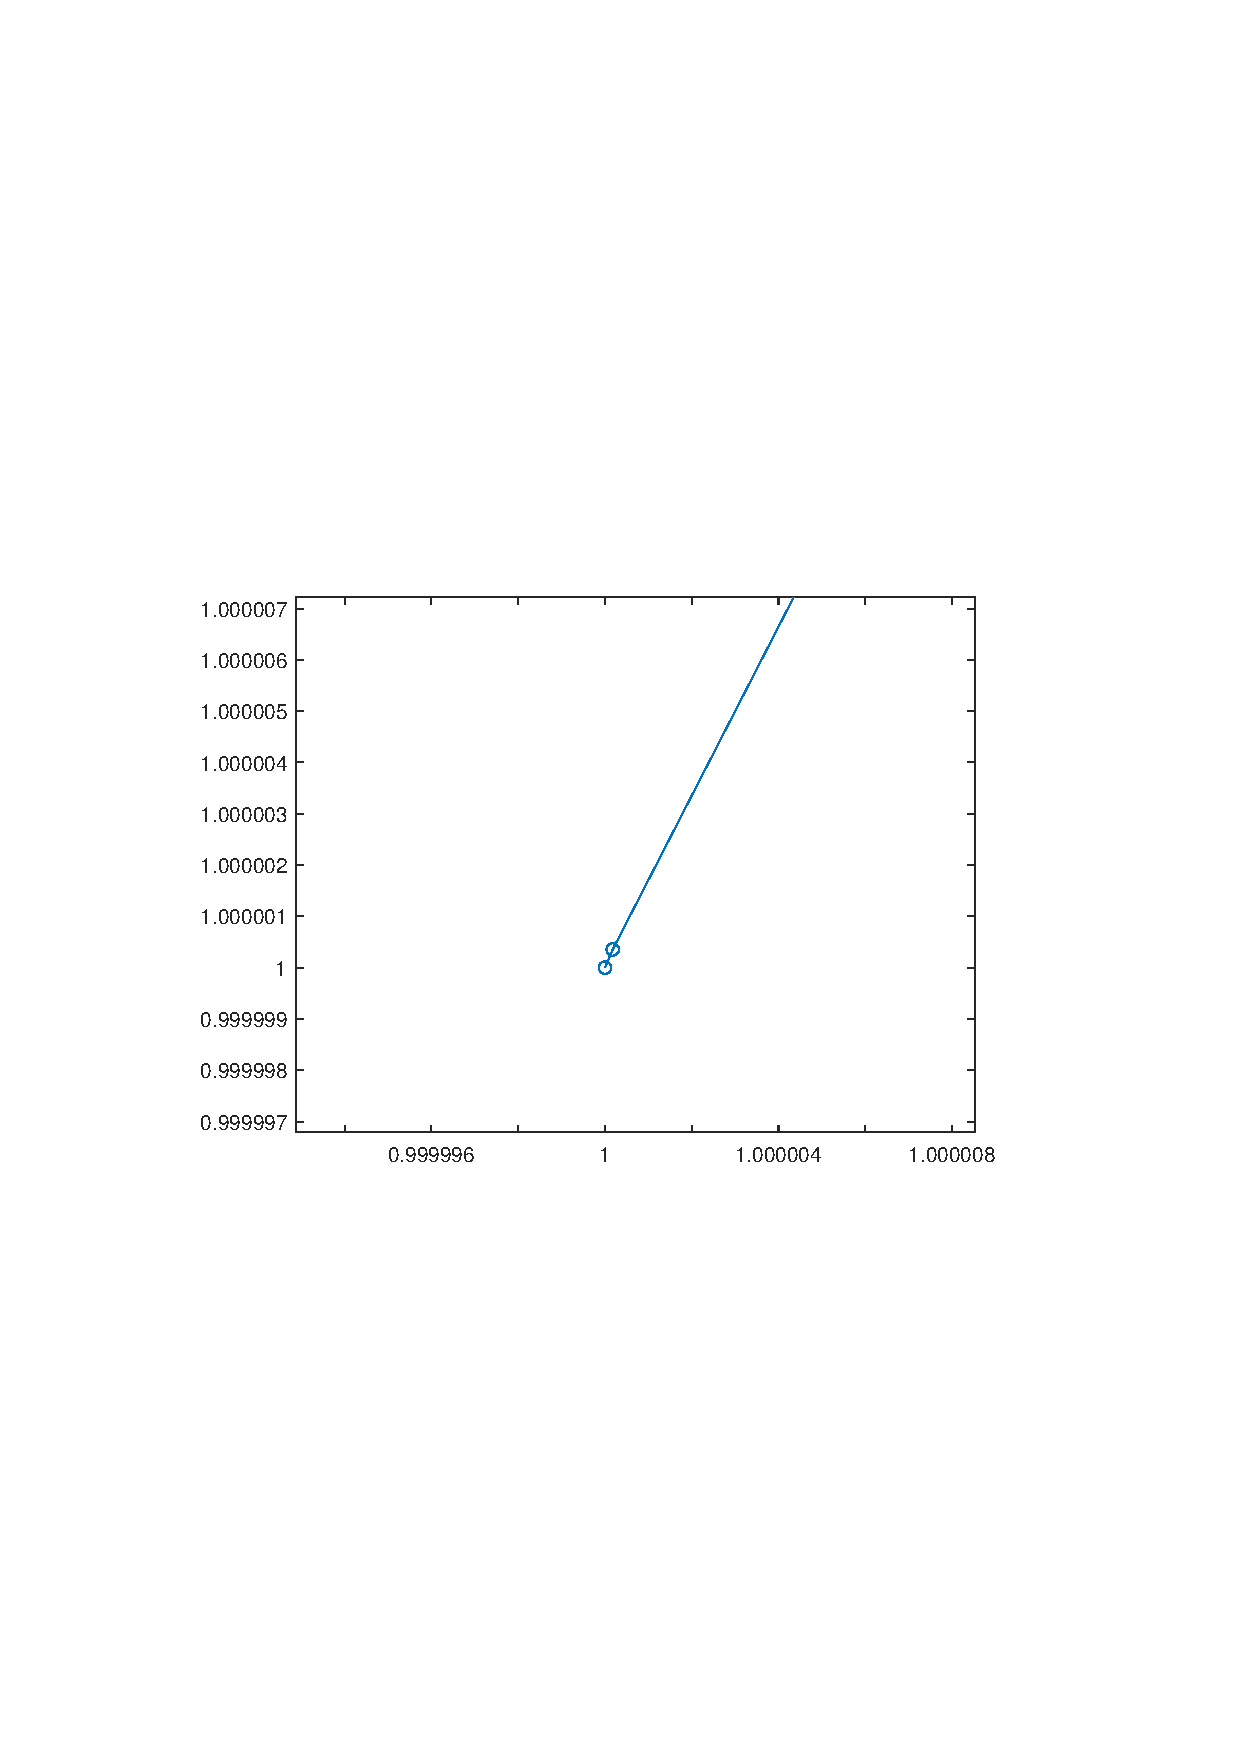
\includegraphics[width=5.3cm]{fig/3_4.pdf}}
\caption{Newton-Armijo in (1.2,1.2)}
\label{Fig.lable}
\end{figure}

\begin{figure}[H]
\centering
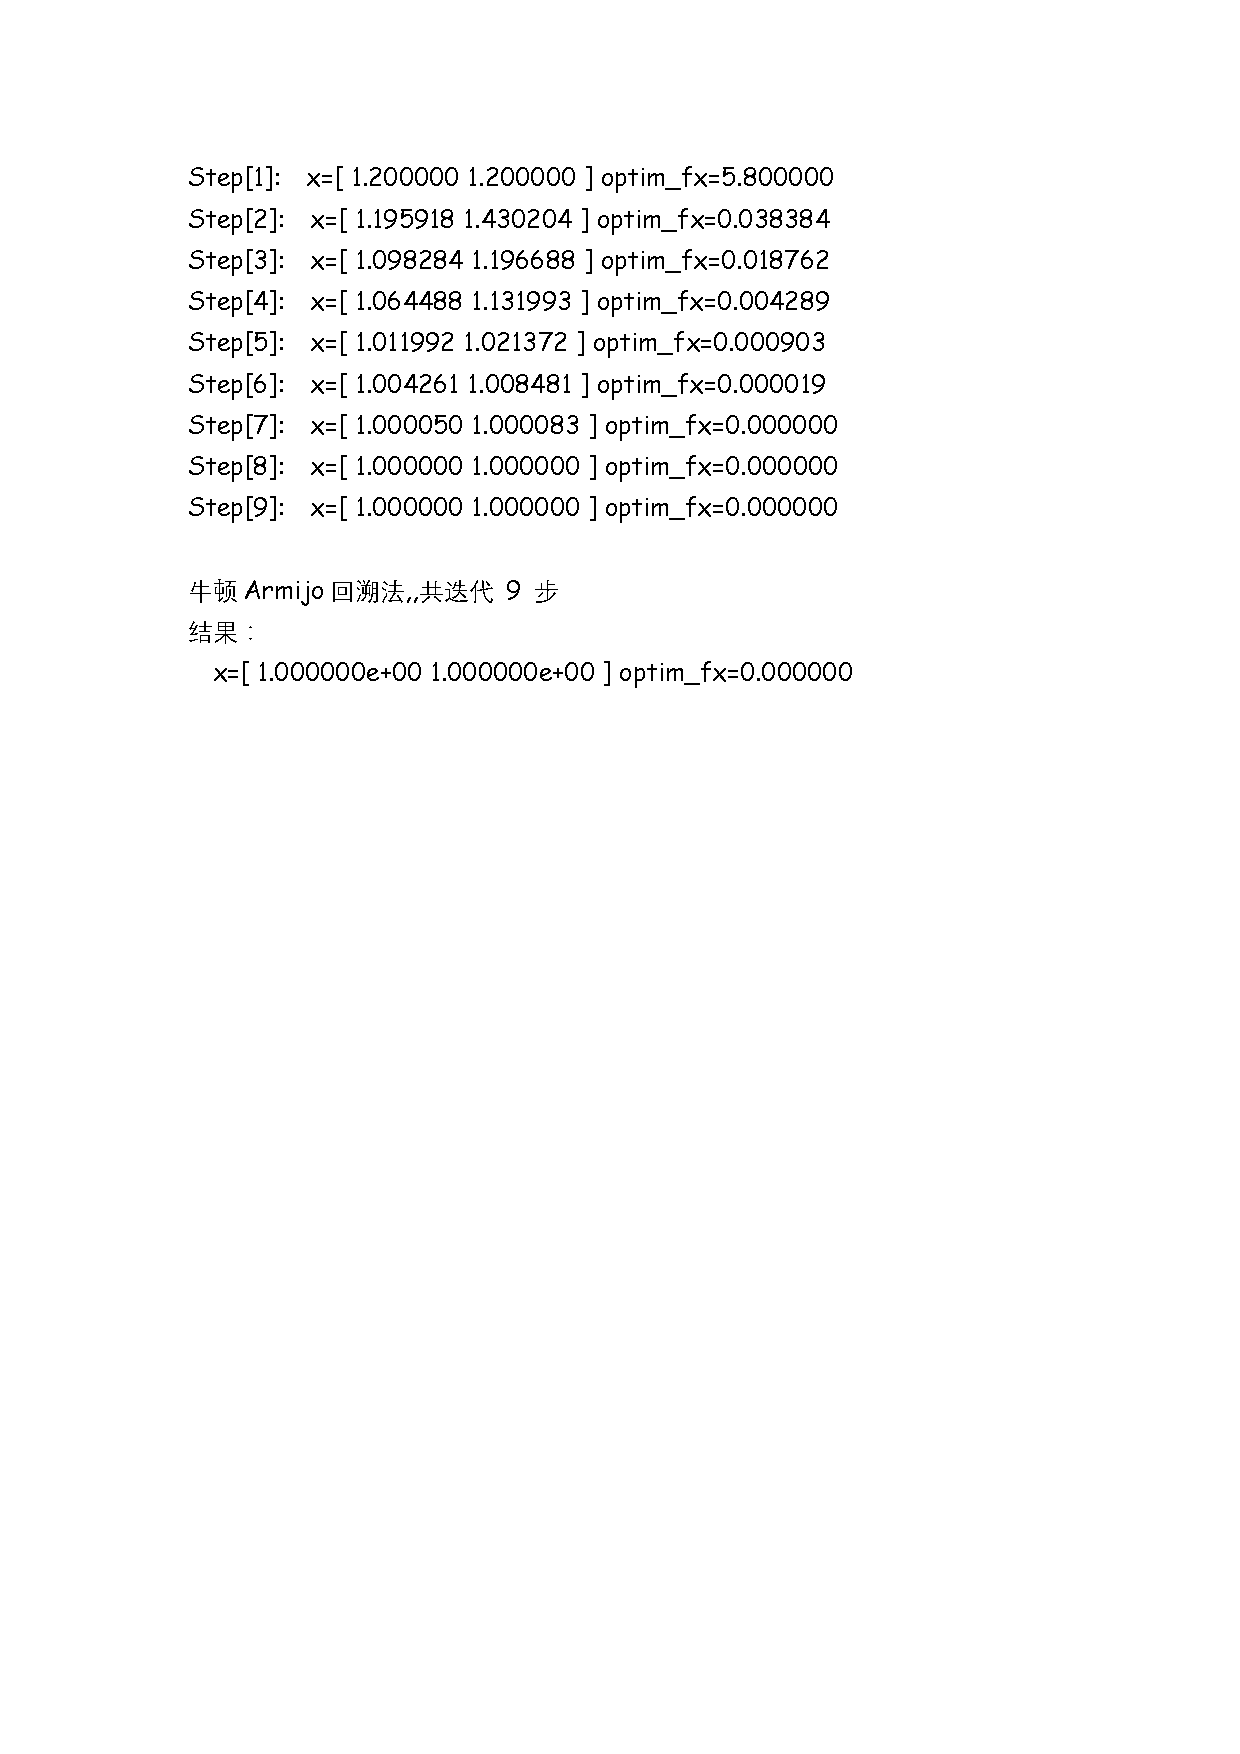
\includegraphics[width=10cm]{fig/3_5.pdf}
%\caption{在$(1,1)$处附近的三维等高线}
\end{figure}

\begin{figure}[H]
\centering
\subfigure{
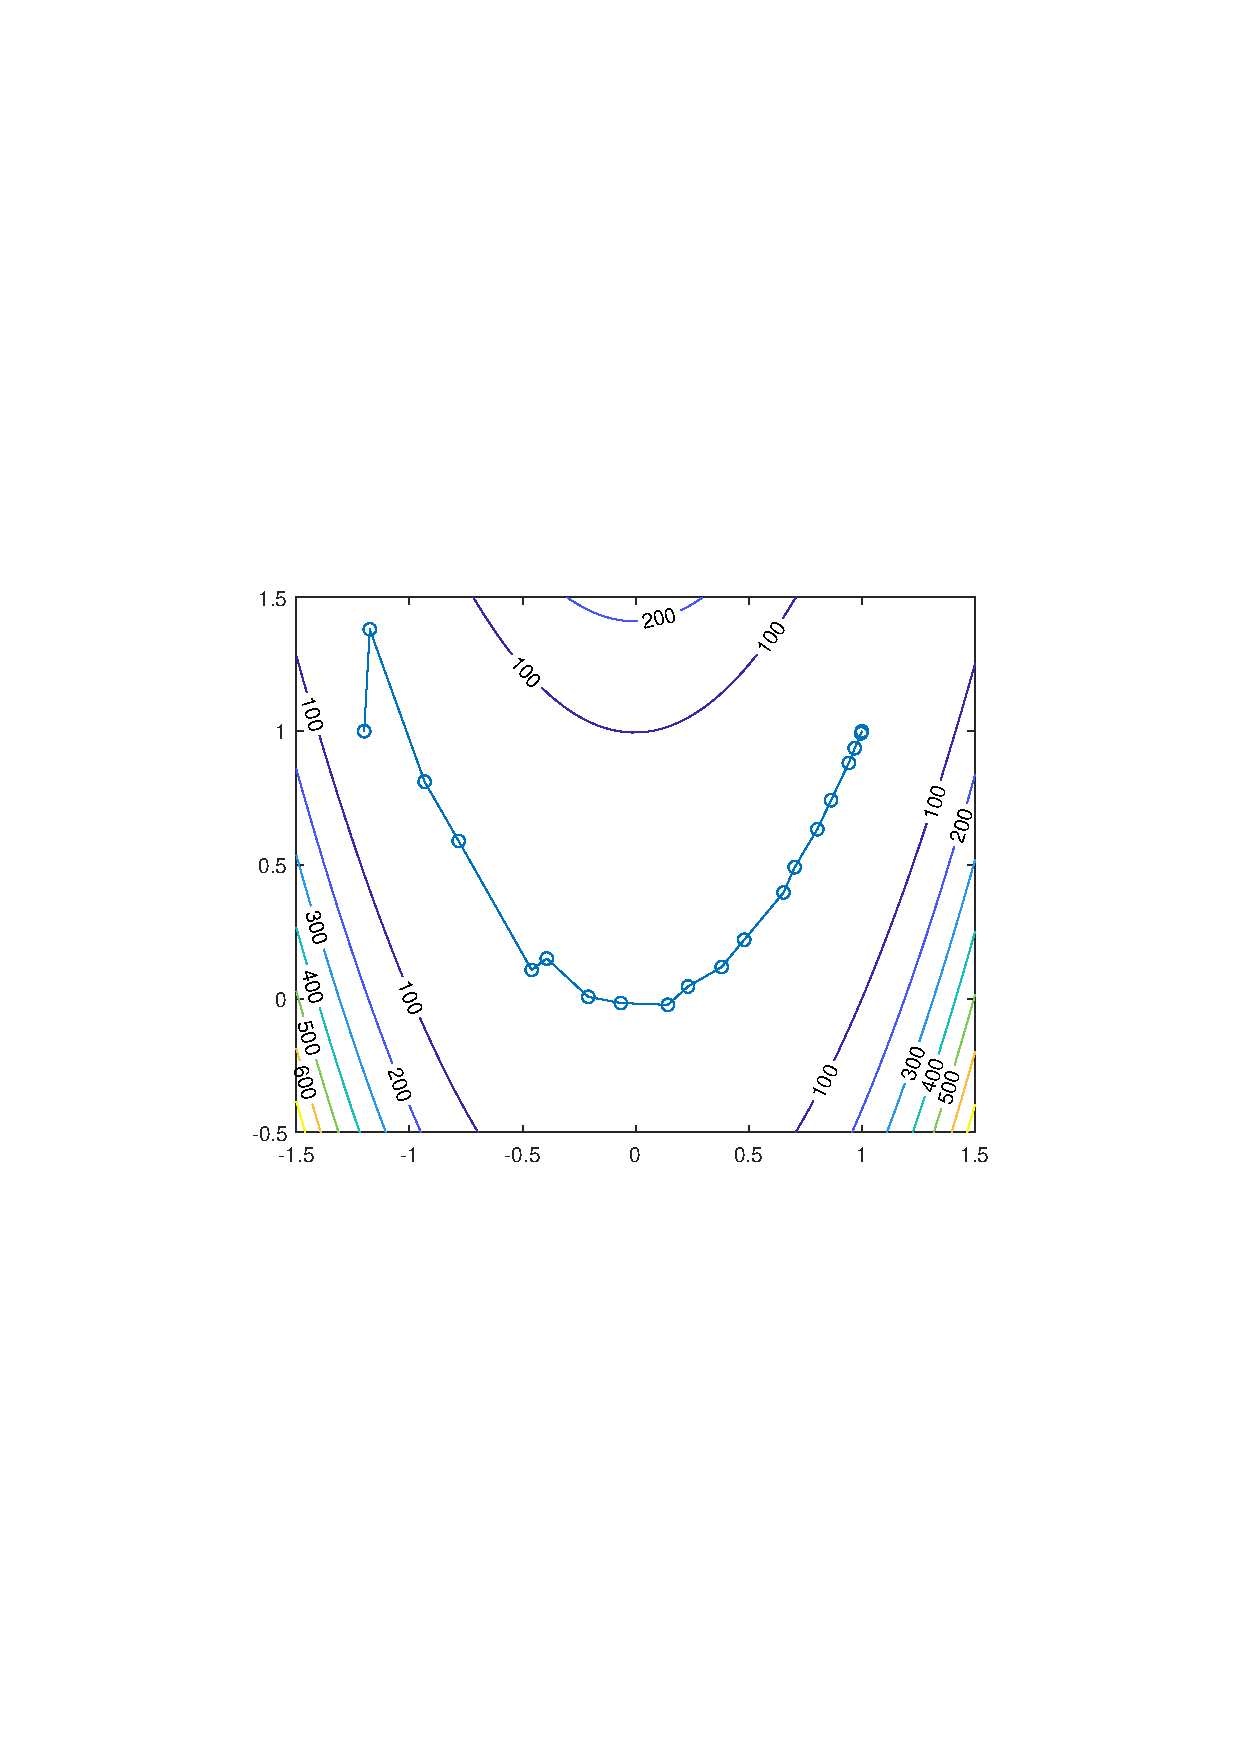
\includegraphics[width=5cm]{fig/4_1.pdf}}
\subfigure{
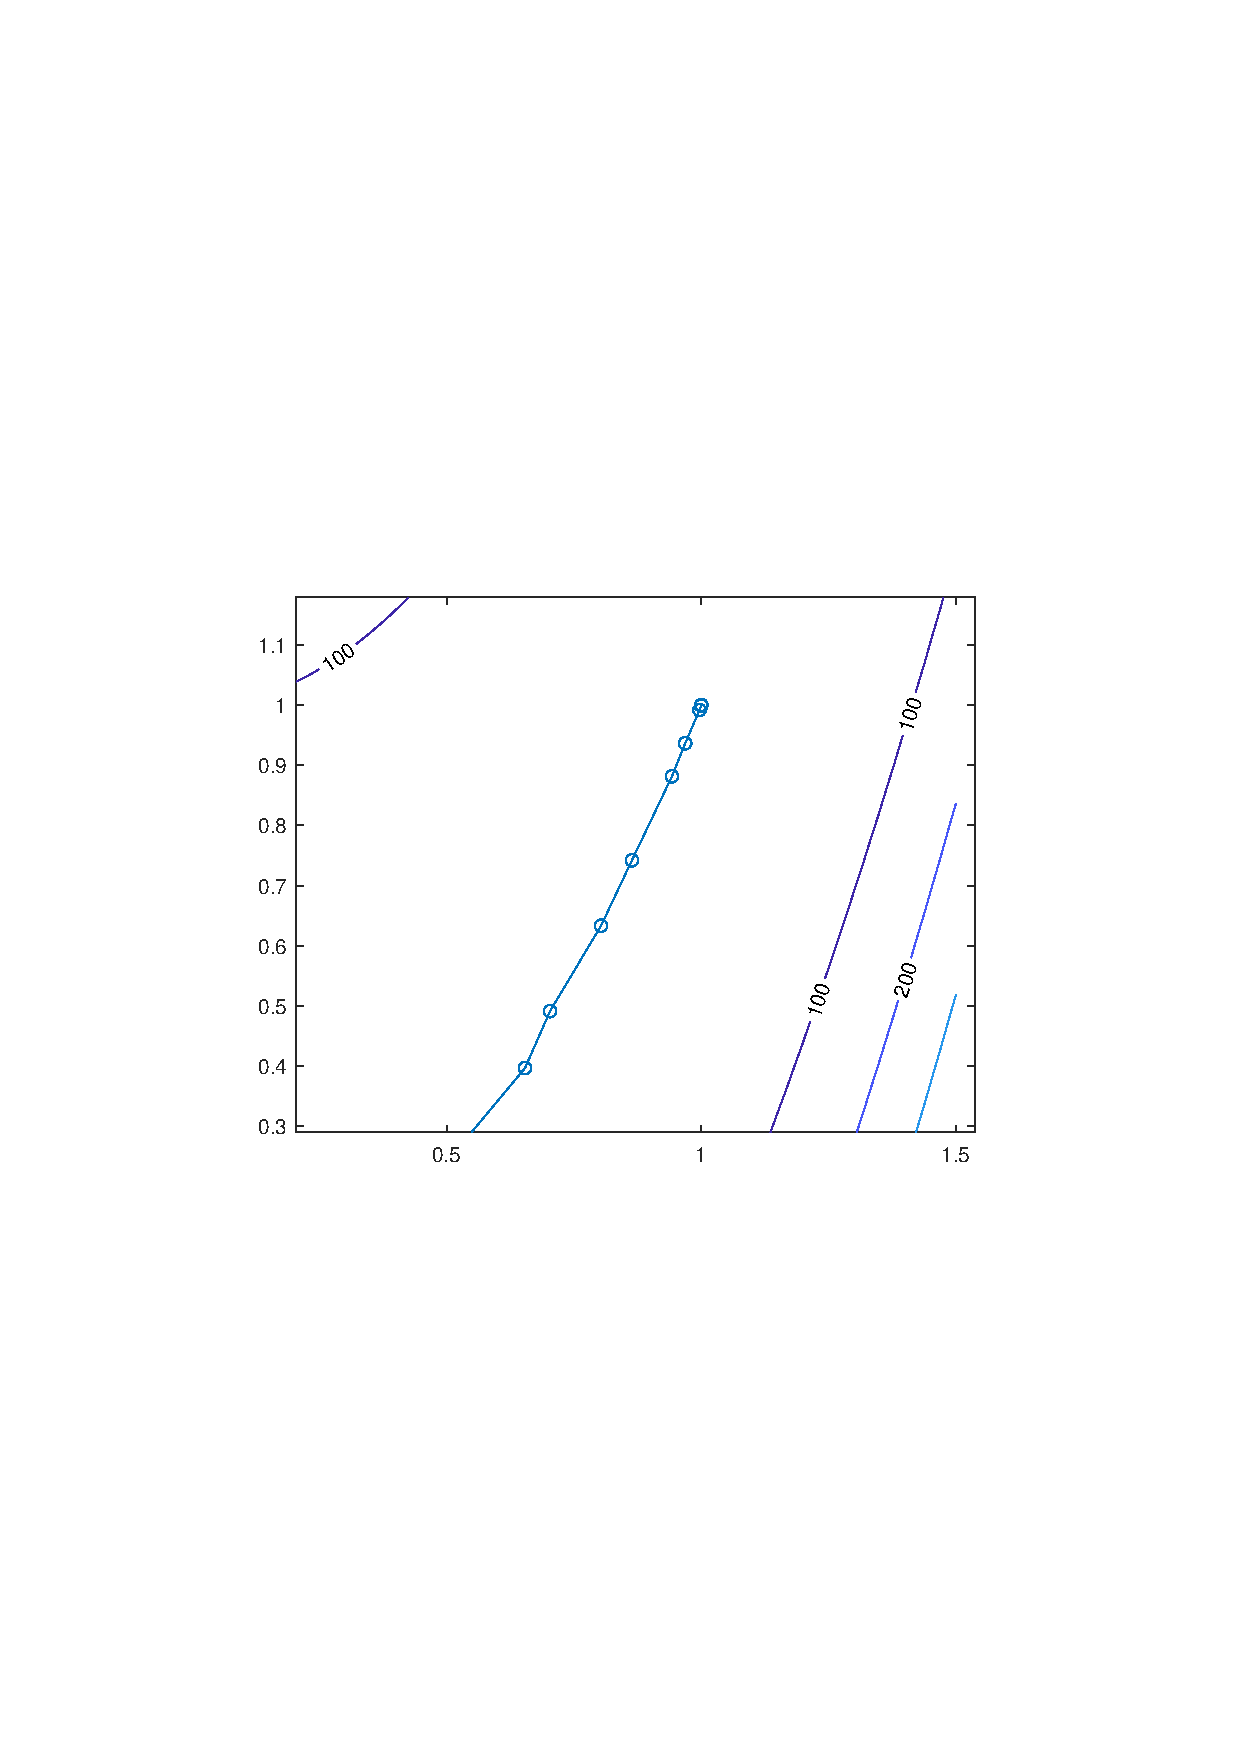
\includegraphics[width=5cm]{fig/4_2.pdf}}
\subfigure{
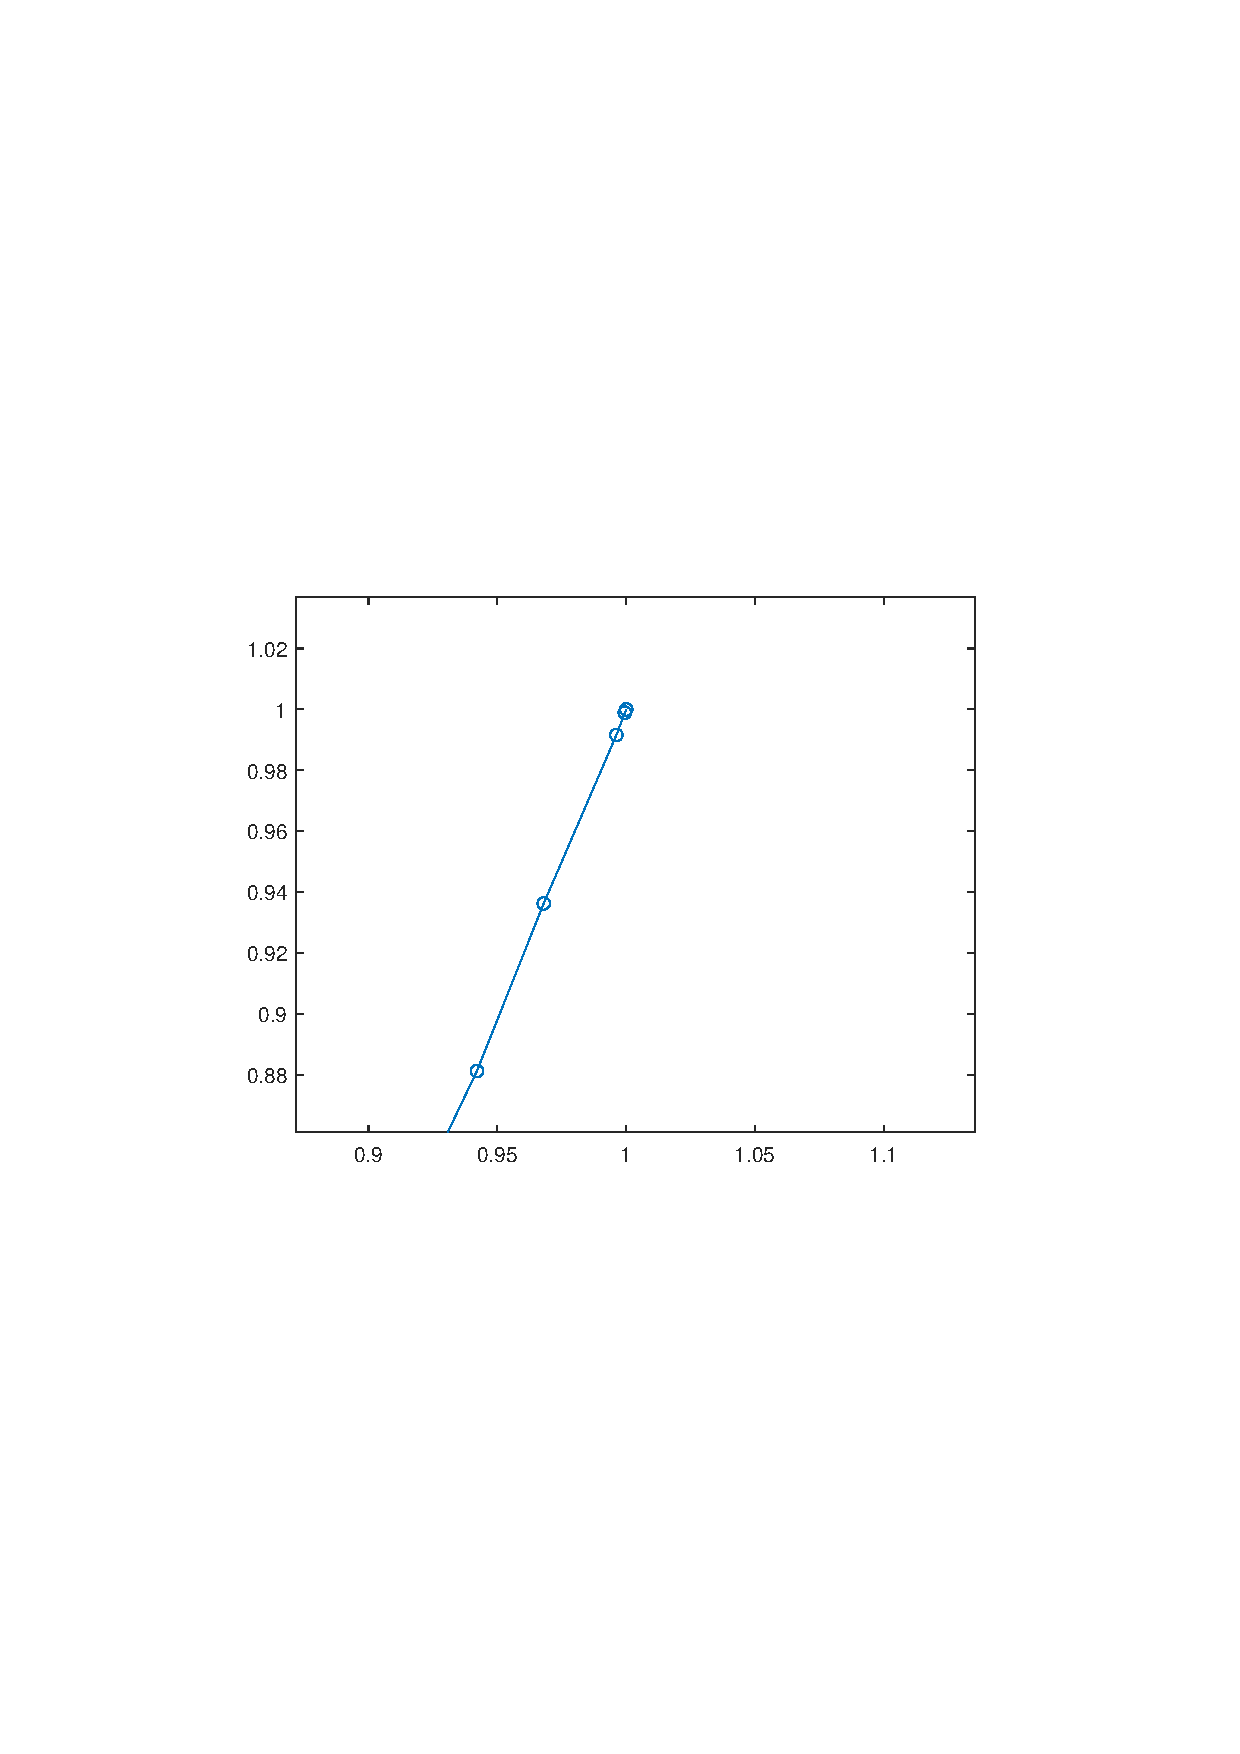
\includegraphics[width=5cm]{fig/4_3.pdf}}
\subfigure{
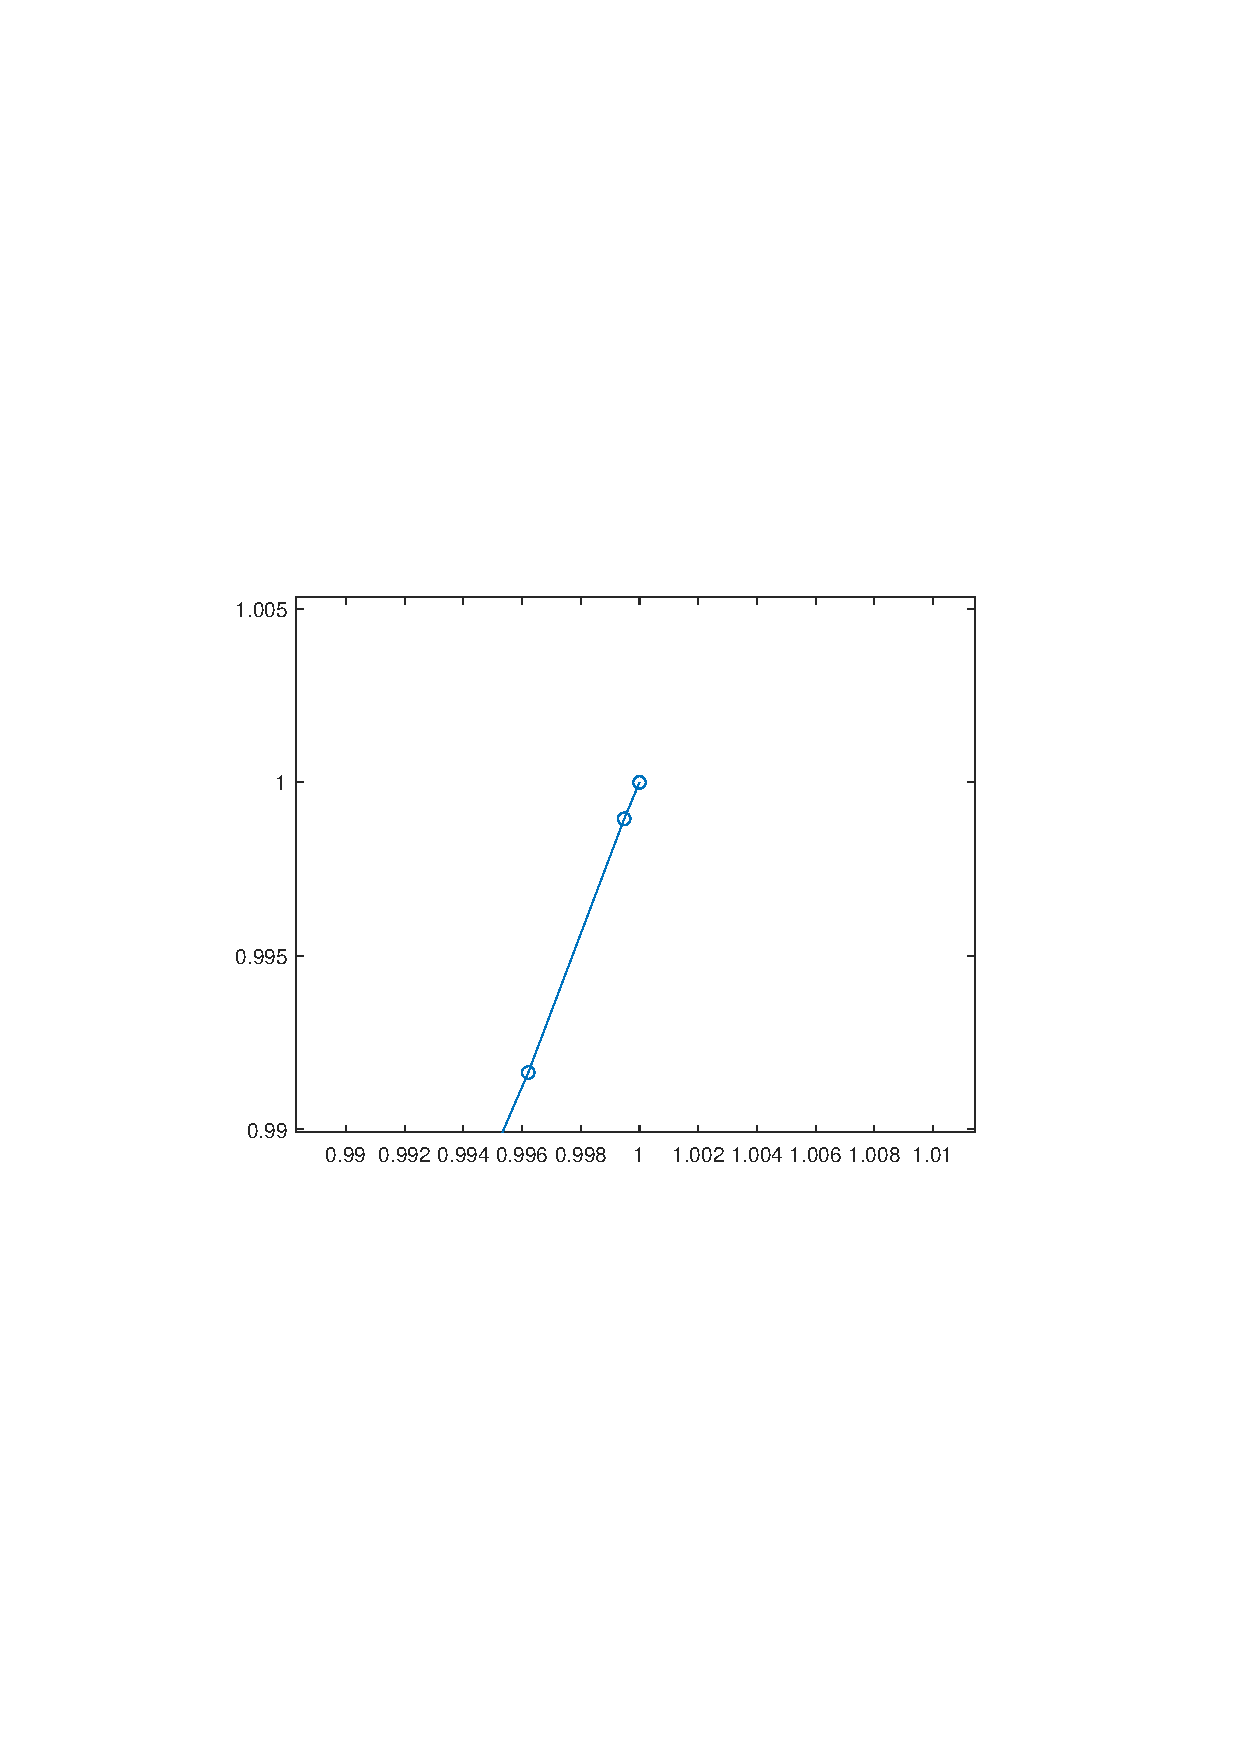
\includegraphics[width=5.3cm]{fig/4_4.pdf}}
\caption{Newton-Armijo in (-1.2,1)}
\label{Fig.lable}
\end{figure}

\begin{figure}[H]
\centering
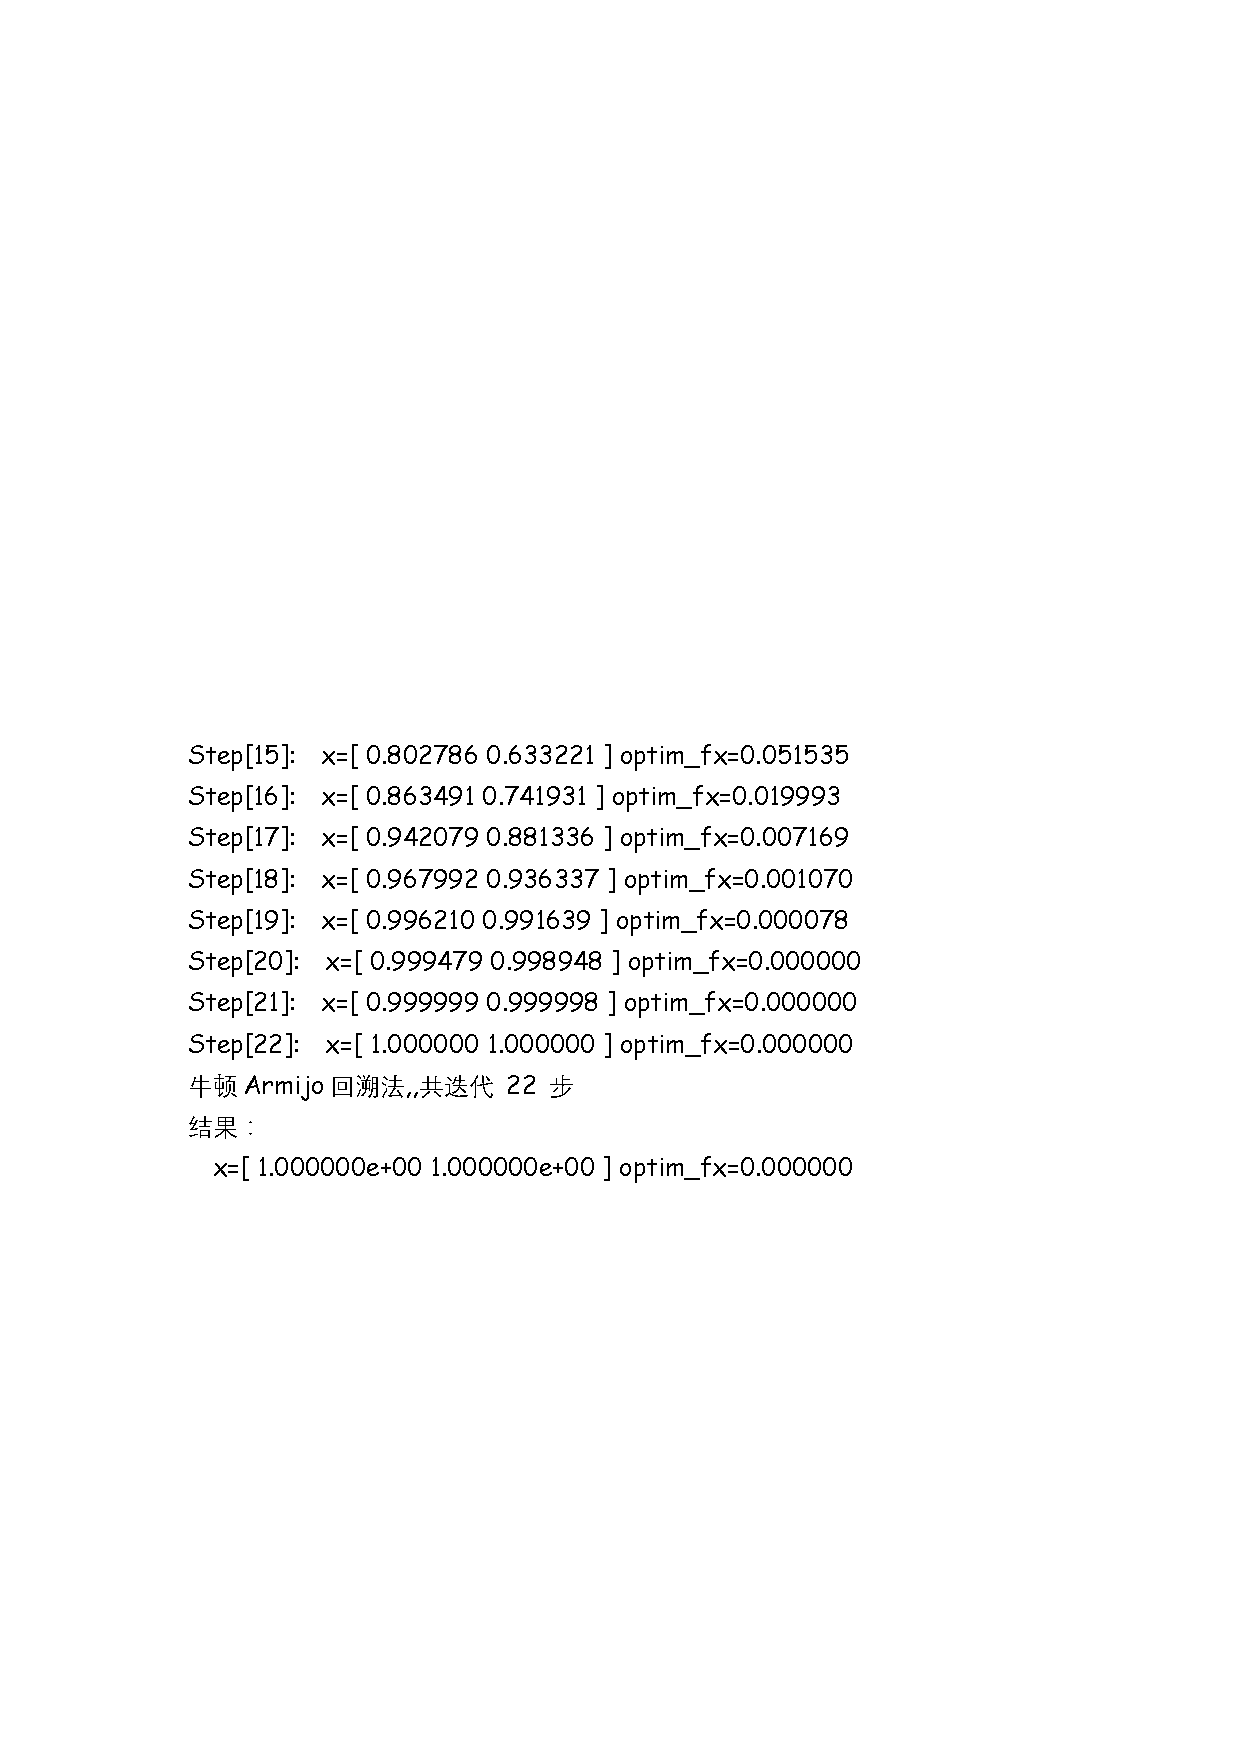
\includegraphics[width=10cm]{fig/4_5.pdf}
%\caption{在$(1,1)$处附近的三维等高线}
\end{figure}

\newpage
\item[5.19] 迭代次数和求解的值如下:

\begin{table}[htbp]
  \centering
  \rowcolors{2}{blue!15}{blue!30}
    \begin{tabular}{cccc}
    \rowcolor{gray!50}
    \textbf{n=5} & \textbf{n=8} & \textbf{n=12} & \textbf{n=20} \\
    \rowcolor{lightgray!50}
    k=6   & k=19  & k=35  & k=66 \\
    \rowcolor{gray!50}
    x     & x     & x     & x \\
    5.00E+00 & 5.90E-11 & -9.61E+00 & -1.10E+01 \\
    -1.20E+02 & -6.97E-11 & 8.15E+02 & 1.05E+03 \\
    6.30E+02 & -5.16E-10 & -1.65E+04 & -2.40E+04 \\
    -1.12E+03 & 1.12E-09 & 1.36E+05 & 2.20E+05 \\
    6.30E+02 & 3.17E-10 & -5.36E+05 & -9.65E+05 \\
          & -6.55E-10 & 1.03E+06 & 1.99E+06 \\
          & -6.57E-10 & -6.43E+05 & -1.25E+06 \\
          & 4.59E-10 & -6.58E+05 & -1.34E+06 \\
          &       & 8.04E+05 & 8.83E+05 \\
          &       & 6.63E+05 & 1.69E+06 \\
          &       & -1.24E+06 & 3.88E+05 \\
          &       & 4.66E+05 & -1.31E+06 \\
          &       &       & -1.71E+06 \\
          &       &       & -5.28E+05 \\
          &       &       & 1.21E+06 \\
          &       &       & 2.00E+06 \\
          &       &       & 9.45E+05 \\
          &       &       & -1.43E+06 \\
          &       &       & -2.65E+06 \\
          &       &       & 1.89E+06 \\
    \end{tabular}%
  \label{tab:addlabel}%
\end{table}%

\newpage
\item[5.21]
\begin{table}[htbp]
  \centering
    \begin{tabular}{cc}
\toprule
    Step  & $x^{(k)}$ \\
		\midrule
    1     &  $(0,0,0,0)$ \\
    2     & $(0.9045, 0,-1.8090,-2.0225)$ \\
    3     & $(-0.4472,-1.8944,-3.3416,-2.7889)$ \\
\bottomrule
    \end{tabular}%
  \label{tab:addlabel}%
\end{table}%

\[G=\left(
\begin{array}{cccc}
 2 & -1 & 0 & 0 \\
 -1 & 2 & -1 & 0 \\
 0 & -1 & 2 & -1 \\
 0 & 0 & -1 & 2 \\
\end{array}
\right)\]

\[P=\begin{bmatrix}
g\\
G*g\\
G^2*g\\
G^3*g\\
\end{bmatrix}^T=
\begin{bmatrix}
-1&0&2&\sqrt{5}\\
-2&-1&4-\sqrt{5}&2 \sqrt{5}-2\\
-3&\sqrt{5}-4&11-4 \sqrt{5}&5 \sqrt{5}-8\\
-\sqrt{5}-2&6 \sqrt{5}-16&34-14 \sqrt{5}&14 \sqrt{5}-27\\
\end{bmatrix}\]

计算MatrixRank[P]=2,故可知其独立向量只有两个
\end{enumerate}

\newpage
\section*{附录代码}
\begin{lstlisting}[language=Octave]
%绘制Rosenbrock函数图形
x=[-8:1:8];  
y=x;  
[X,Y]=meshgrid(x,y);  
[row,col]=size(X);  
for l=1:col  
    for h=1:row  
        z(h,l)=Rosenbrock([X(h,l),Y(h,l)]);  
    end  
end  
surf(X,Y,z);  
shading interp  

function result=Rosenbrock(x)  
%Rosenbrock 函数  
%输入x,给出相应的y值,在x=(1,1) 处有全局极小点0,为得到最大值,返回值取相反数   
[row,col]=size(x);  
if row>1  
    error('输入的参数错误');  
end  
result=100*(x(1,2)-x(1,1)^2)^2+(x(1,1)-1)^2;  
result=-result;  
end
\end{lstlisting}

\begin{lstlisting}[language=Octave]
%本实验采用最速下降法,步长为精确步长,测试函数为Rosenbrock函数
%%
%用符号表达式定义目标函数
clc;
clear;
syms x1 x2;
X=[x1,x2];
f=100*(X(2)-X(1)^2)^2+(1-X(1))^2;
F=eval(['@(x1,x2)',vectorize(f)]);
fx=diff(f,x1); %求f对x1偏导数
fy=diff(f,x2); %求f对x2偏导数
fxx=diff(fx,x1); %求二阶偏导数 对x1再对x1
fxy=diff(fx,x2); %求二阶偏导数 对x1再对x2
fyx=diff(fy,x1); %求二阶偏导数 对x2再对x1
fyy=diff(fy,x2); %求二阶偏导数 对x2再对x2
Gradient=[fx;fy];     %计算梯度表达式
Hesse=[fxx,fxy;fyx,fyy];
x=[-1.2,1];        %定义初始点

%%
N=200;     %总迭代次数
e=0.000001;
P=zeros(N,2);    %储存点的轨迹
OPT=zeros(N,2);     %储存最优值下降的轨迹
g=subs(Gradient,[x1 x2],[x(1) x(2)]);
step=1;
P(step,:)=x;
optim_fx=subs(f,[x1 x2],[x(1) x(2)]);
fprintf('Step[%d]:  x=[ %f %f ] optim_fx=%f\n',step,x(1),x(2),double(optim_fx));
OPT(step,:)=optim_fx;
%%
while (norm(g)>e  && step < N)       %当g的2-范数小于特定值时,或迭代次数到达上限时,停止迭代
    step=step+1;
    %计算目标函数点x(k)处一阶导数值
    g=subs(Gradient,[x1 x2],[x(1) x(2)]);
    %计算目标函数点x(k)处Hesse矩阵
    G=subs(Hesse,[x1 x2],[x(1) x(2)]);
    %计算目标函数点x(k)处搜索方向p
    %p=-G\g';
    p=-g;
    %点x(k)处的搜索步长
   
    ak=1;
   % ak=Alpha(p,g,G);
    xk=x+ak*double(p');
    %采用Armijo法则计算近似步长ak
    while(F(xk(1),xk(2)) > (F(x(1),x(2))+0.1*double(p'*g)*ak))
        ak=0.5*ak;
        xk=x+ak*double(p');
    end
    x=x+double(ak*p');
    %输出结果
    optim_fx=subs(f,[x1 x2],[x(1) x(2)]);
    fprintf('Step[%d]:  x=[ %f %f ] optim_fx=%f\n',step,x(1),x(2),double(optim_fx));
    P(step,:)=x;
    OPT(step,:)=optim_fx;
    g=subs(Gradient,[x1 x2],[x(1) x(2)]);
end
%输出结果
optim_fx=subs(f,[x1 x2],[x(1) x(2)]);
fprintf('\n最速下降法,共迭代 %d 步\n结果:\n  x=[ %d %d ] optim_fx=%f\n',step,x(1),x(2),double(optim_fx));
P(step+1:N,:)=[];      %删去P中的多余空间\
figure;
plot(P(:,1),P(:,2))
hold on;
xx =linspace(-1.5,1.5);
yy = linspace(-0.5,1.5);
[X,Y] = meshgrid(xx,yy);
Z=F(X,Y);
contour(X,Y,Z,'ShowText','on')
figure;
plot(OPT)
%%
% 最速下降法子程序,计算精确步长ak
function a=Alpha(p,g,G)
a=-(p'*g)/(g'*G*g);
a=double(a);
end
\end{lstlisting}

\begin{lstlisting}[language=Octave]
%牛顿Armijo回溯法
%%
%用符号表达式定义目标函数
clc;
clear;
syms x1 x2;
X=[x1,x2];
f=100*(X(2)-X(1)^2)^2+(1-X(1))^2;

F=eval(['@(x1,x2)',vectorize(f)]);
fx=diff(f,x1); %求f对x1偏导数
fy=diff(f,x2); %求f对x2偏导数
fxx=diff(fx,x1); %求二阶偏导数 对x1再对x1
fxy=diff(fx,x2); %求二阶偏导数 对x1再对x2
fyx=diff(fy,x1); %求二阶偏导数 对x2再对x1
fyy=diff(fy,x2); %求二阶偏导数 对x2再对x2
Gradient=[fx;fy];     %计算梯度表达式
Hesse=[fxx,fxy;fyx,fyy];
x=[-1.2,1];        %定义初始点

%%
N=100;     %总迭代次数
e=0.000001;
P=zeros(N,2);    %储存点的轨迹
OPT=zeros(N,2);     %储存最优值下降的轨迹
g=subs(Gradient,[x1 x2],[x(1) x(2)]);
step=1;
P(step,:)=x;
optim_fx=subs(f,[x1 x2],[x(1) x(2)]);
fprintf('Step[%d]:  x=[ %f %f ] optim_fx=%f\n',step,x(1),x(2),double(optim_fx));
OPT(step,:)=optim_fx;
%%

while (norm(g)>e  && step < N)       %当g的2-范数小于特定值时,或迭代次数到达上限时,停止迭代
    step=step+1;
    %计算目标函数点x(k)处一阶导数值
    g=subs(Gradient,[x1 x2],[x(1) x(2)]);
    %计算目标函数点x(k)处Hesse矩阵
    G=subs(Hesse,[x1 x2],[x(1) x(2)]);
    %计算目标函数点x(k)处搜索方向p
    p=-inv(G)*g;
    %p=-g;
    %点x(k)处的搜索步长
    %ak=Alpha(p,g,G);
    %ak=1;
    ak=1;
    xk=x+ak*double(p');
    %采用Armijo法则计算近似步长ak
    while(F(xk(1),xk(2)) > (F(x(1),x(2))+0.01*double(p'*g)*ak))
        ak=0.5*ak;
        xk=x+ak*double(p');
    end
    x=x+double(ak*p');
    %输出结果
    optim_fx=subs(f,[x1 x2],[x(1) x(2)]);
    fprintf('Step[%d]:  x=[ %f %f ] optim_fx=%f\n',step,x(1),x(2),double(optim_fx));
    P(step,:)=x;
    OPT(step,:)=optim_fx;
    g=subs(Gradient,[x1 x2],[x(1) x(2)]);
end
%输出结果
optim_fx=subs(f,[x1 x2],[x(1) x(2)]);
fprintf('\n牛顿Armijo回溯法,,共迭代 %d 步\n结果:\n  x=[ %d %d ] optim_fx=%f\n',step,x(1),x(2),double(optim_fx));
P(step+1:N,:)=[];      %删去P中的多余空间
figure;
plot(P(:,1),P(:,2),'-o')
hold on;
xx =linspace(-1.5,1.5);
yy = linspace(-0.5,1.5);
[X,Y] = meshgrid(xx,yy);
Z=F(X,Y);
contour(X,Y,Z,'ShowText','on')
figure;
plot(OPT)
%%
% 计算精确步长ak
function a=Alpha(p,g,G)
    a=-(p'*g)/(p'*G*p);
end

%采用Armijo法则计算近似步长ak
function a=Armijo(x,p,g)
    a=1;
    xk=x+a*double(p);
    while(F(xk(1),xk(2)) > F(x(1),x(2))+0.01*doubel(p'*g)*a)
        a=0.9*a;
        xk=xk+a*double(p);
    end
end
\end{lstlisting}

\begin{lstlisting}[language=Octave]
%Conj_Grad  共轭梯度法
clc;
clear;
N=4;
G=zeros(N,N);
b=[-1,0,2,5^(0.5)]';
x0=zeros(N,1);
for i= 1:N
     G(i,i) = 2;
end

for i= 1:N-1
    G(i+1,i)=-1;
    G(i,i+1)=-1;
end
    x = x0;x'
    g = G*x+b;
    p = -g;
    k = 0;
    while 1
        if norm(g, 2)<1e-6
            break
        end
        k = k + 1;
        
        d=G*p;
        a=(g'*g)/(p'*d);

        x = x+a*p;x'
        t=g+a*d;
       beta=(t'*t)/(g'*g);
       g=t;
       p=-g+beta*p;
  
    end
\end{lstlisting}
\end{document}

